\documentclass[12pt]{article}
%\usepackage[showframe]{geometry}% http://ctan.org/pkg/geometry
\usepackage{lipsum}% http://ctan.org/pkg/lipsum
\usepackage{multicol}% http://ctan.org/pkg/multicols
\usepackage{graphicx}% http://ctan.org/pkg/graphicx
\usepackage{float}
\usepackage{fancyhdr}
\usepackage{titling}
\usepackage{subcaption}
\usepackage{indentfirst}
\usepackage{booktabs}
\usepackage{multirow} 
\usepackage{setspace} \doublespacing
\usepackage{mathptmx}
\usepackage{amsmath}
\usepackage[backend=biber, style=apa,]{biblatex}
\usepackage{hyperref}
\usepackage{float}
\usepackage{caption}
\usepackage{sectsty}
\usepackage{titlesec} % Add titlesec package

\pagestyle{fancy}
\doublespacing

%\addbibresource{/mnt/c/Users/woute/projects/Thesis_endstop/MyLibrary.bib}
% \addbibresource{/home/wouter/projects/Thesis_endstop/latex_endstop/MyLibrary.bib}
\addbibresource{MyLibrary.bib}

\hyphenpenalty=1000
\tolerance=2000

\fancyhead{}
\fancyfoot{}
\fancyfoot[R]{\thepage}
\renewcommand{\headrulewidth}{0pt}

% Adjust header whitespace
\setlength{\headheight}{5pt}  % Adjust as needed
\setlength{\headsep}{5pt}     % Adjust as needed

\setlength{\droptitle}{-10em}   % This is your set screw
\setlength{\parindent}{0pt}

\sectionfont{\large} % Change \Large to your desired size
%\subsectionfont{\normalsize} % Change \large to your desired size

% Center the section titles
\titleformat{\section}
  {\normalfont\Large\bfseries\filcenter} % Format: font size, weight, alignment
  {\thesection}{1em}{} % Label and separation from title

\begin{document}

\captionsetup{font=small}

\begin{titlepage}
\centering

% Adjust font size and family as needed
{\LARGE\bfseries Hierarchical Circuit Structure of Mouse Visual Cortex for Generating Illusory Contour Responses\par}

\vspace{5pt} % Adjust space between title and figure as needed

% Include the figure

\includegraphics[width=0.5\textwidth]{figures/donders_logo.png}

\includegraphics[width=0.5\textwidth]{figures/uva_logo.png}

\vspace{20pt} % Adjust space between figure and author/date as needed

% Author and Date
{\Large Wouter Kroot\par}
\vspace{5pt} % Adjust as needed
{\Large April 2024\par}
\vspace{5pt}
{\Large Supervisor: Prof. dr. P.H.E. Tiesinga}

\end{titlepage}

% Rest of the document starts here
\newpage

% Abstract
\begin{abstract}
  \footnotesize
  Recent insights into mice physiology demonstrated their ability to perceive illusory contours and identifying the significance of recurrent processing in complex visual perception. Together with computational work that demonstrated that length tuned endstopped cells can effectively be used to delineate visual boundaries, particularly in environments with ambiguous or occluded objects. We aimed to simulate illusory contours to better understand the contribution of recurrent activity to illusory contour representation in primary visual cortex. We developed a Leaky Integrate and Fire (LIF) model, along with population firing rate models, to simulate the spatial and temporal dynamics necessary for stable endstopping and to demonstrate how these specifc endstopped cells facilitate the representation of illusory contours through recurrent activity. Our findings indicate that orientation-selective and length-tuned endstopped cells are crucial for detecting features that induce illusory contours. Additionally, we demonstrated that when endstopped endzones are modulated by indirect inhibitory feedback mechanisms, stability is maintained when input deviates from the optimal orientation. These cells are shown to converge in higher visual areas, such as the lateromedial (LM) area, where they integrate local cues to generate perceptual boundaries corresponding to illusory contours. These boudaries are then significantly amplified through feedback pathways and an illusory occluding figure is lifted from the inducers. Our models not only underscore the functionality of endstopped cells in inferential visual processing but also highlight the potential of using mice as effective models to explore cortical architectures comparable to those in primates, supporting broader implications for understanding cortical organisation across species.
\end{abstract}

% \newpage
% {\scriptsize
% \tableofcontents}

\newpage
\section*{Introduction}
% a paragraph is around 200 -300 words containing: 

% - Begin with a topic sentence that clearly states the main point or focus of the paragraph. Sets direction and tone informing content and how it relates the the main question or thesis.

% - Necessary background information including definitions a breif review of relevant literature or disucssion of how issue has been approached in the field.

% - Evidence that support point such as data and quantification. substantiates your claims but also shows engagement with tthe existing body of knowledge

% - Analysis of what this evidence means, discuss meaning in the context of my work.

% - Concluding sentence that ties the evidence to the next paragraph. Use: forecasting hinting at the next topic, Linking using literally connecting them with: Furthermore, Additionally, in contrast. 

%------------------------------------------------------------------------------------------------
% Visual image segmentation and illusory contours

%\subsection{Recurrent activity is essential for robust image segmentation.}

\setlength{\parindent}{24pt}
The mammalian visual system is a complex network of interconnected areas that together process external inputs, information enters as two dimensional retinal signals and are transfomred into a coherent three-dimensional representation in the cortex. An essential part of this process is the ability to segment visual scenes into object distinct from their background and other objects \autocite{kirchbergerEssentialRoleFeedback2020}. Early visual areas, such as the primary visual cortex (V1), perform a local analysis of visual features with relatively small receptive fields and feed their output to higher visual areas (HVAs) that integrate that information over a larger spatial extent and process increasingly abstract features such as object category \autocite{ashbridgeEffectImageOrientation2000}. Visual input in V1 is often clearly defined, e.g., by a luminance contrast that indicates a discontinuity such as an edge or a corner. In other cases, feedforward information is more ambiguous or incomplete and requires further processing for a robust global representation. For example, when an object is occluded by another object, the visual system must make perceptual inferences about the occluded figure and have to fill in the missing details. Interestingly, particular stimulus configurations can induce the perception of an occluding figure while no occluding contour is physically present, these are also known as illusory contours \hyperref[fig:figure_1]{(Figure 1a and b)}. Because these illusory contours are a direct product of the underlying neural circuitry, they can effectively be used to investigate the neurophysiological interactions required to make visual inferences such as illusory contours. Hypotheses suggest that filling in missing visual information involves recurrent processing between lower visual areas and higher visual areas (HVAs) \autocite{wyatteEarlyRecurrentFeedback2014}. Furthermore, recurrent connectivity, which includes both horizontal connections within a visual area and their induced feedback connections, facilitates the integration of local and global visual features, thereby refining visual representations \autocite{roelfsemaCORTICALALGORITHMSPERCEPTUAL2006,shushruthStrongRecurrentNetworks2012}. From this perspective, illusory contours might reflect a process of neural activity filling in contour information in between particular inducing points relayed within the feedforward visual input to generate a superimposed object.
\setlength{\parindent}{0pt}

\bigbreak
%\subsection{Illusory contour representation in the visual cortex.}
Although many stimulus configurations make it possible to induce the perception of illusory contours, they often share common features \autocite{palmerLateInfluencesPerceptual2000}. Consider the abutting grating illusion \autocite{sorianoAbuttingGratingIllusion1996} and the Kanizsa triangle illusion \autocite{kanizsaSubjectiveContours1976}. Both illusions involve extrapolations from visual cues that suggest the presence of an occluding object. In the Kanizsa triangle illusion, three pacman-shaped figures are arranged such that a continuous contour seems to connect the edges of the inducers \hyperref[fig:figure_1]{(figure 1a)}. Similarly, in the abutting grating illusion, the vertical alignment of horizontal lines creates the impression of a vertical contour superimposed on horizontal inducers \hyperref[fig:figure_1]{(figure 1 b)}. In both illusions inducer input consist of seemingly simple geometrical forms, however, for the resulting figure to emerge from the background inducers, they require sophisticated processing of individual inducer shapes. Namely, their position and orientation need to be processed in relation to each other. This inter-object complexity necessitates the integration of segmented stimuli, possibly involving feedback or recurrent activity. Single-unit recordings from cats and primates have identified particular neurons in the early visual cortex that react to subjective contours similar to how they respond to real lines \autocite{leeDynamicsSubjectiveContour2001,vonderheydtMechanismsContourPerception1989}. Notably, the response times in the secondary visual area (V2) precede those in V1. Indicating that the first place sensitivity to illusory contours arises in the rhesus macaque is V2. Recurrent processing has been demonstrated to be an important part of the perceptual organisation \autocite{roelfsemaCORTICALALGORITHMSPERCEPTUAL2006}. Recurrent processing can support grouping of behaviourally relevant objects and separating objects from the background. This recirculation of information is associated with synaptic and conduction delays and would fit the times delays observed during the filling in process of illusory contours (55 ms) \autocite{leeDynamicsSubjectiveContour2001,pakTopDownFeedbackControls2020}. If V2 illusory responses are due to recurrent activity and real and illusory contours are processed by the same cells, a direct implication would be that higher visual areas might be unable to distinguish between real and illusory contours.

\begin{figure}[H]
    \centering
    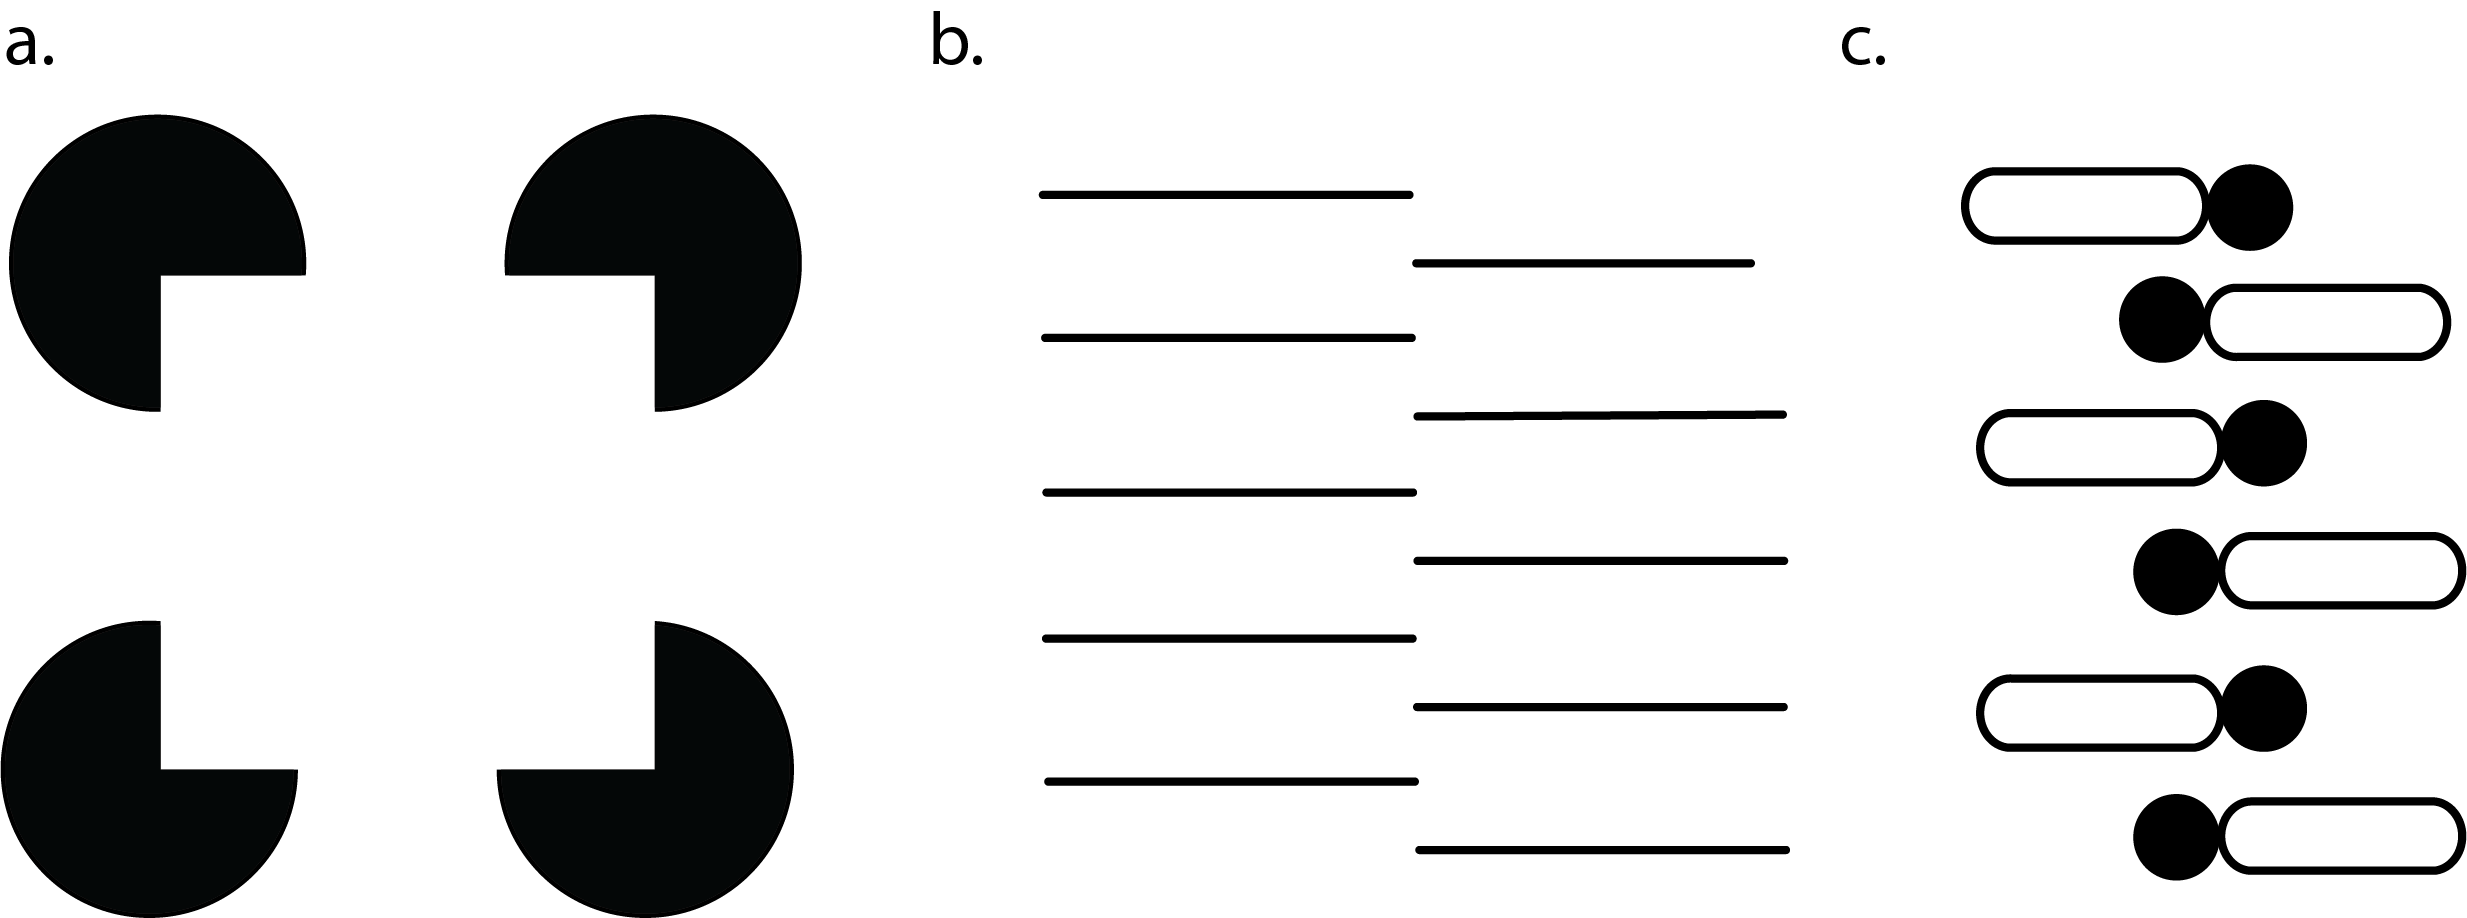
\includegraphics[width=1.0\textwidth]{adjusted_figures/illusory_figure.png}
    \caption{a. The kanizsa illusion \autocite{kanizsaSubjectiveContours1976}. Four pac-man shaped inducers can be perceived as four circles with an overlapping white square. b. The activity elicited in mouse V1 by the Kanizsa triangle. After mapping the receptive fields of a set of neurons the Kanizsa inducers were placed such that the receptive fields of these neurons were not stimulated by feedforward input. Still, the neurons responses were measured due to feedback signals related to the illusory contour.
    c. The Abutting grating illusion \autocite{sorianoAbuttingGratingIllusion1996}. The alignment between the horizontal inducers gives the impression of a vertical contour. d. The proposed neural mechanism for the detection of these visual features are endstopped cells, which can be characterised by an elongated receptive field with an inhibitory endzone.}
    \label{fig:figure_1}
\end{figure}



%ToDo talk about the figure and check whther the references are good
%\subsection{Illusory contours are controlled by top-down projections.}
This hypothesis has been examined, with area V4 in the macaque identified as a crucial integration point where both real and illusory contours are represented equivalently \autocite{panEquivalentRepresentationReal2012}. Through the use of optical imaging and single-cell recordings to compare neural activity elicited by real and illusory contours across areas V1, V2, and V4, it was found that activities in V1 and V2 predominantly relate to the encoding of local spatial features of the inducers, rather than the global orientation of the illusory contour. Meanwhile, V4 processed both real and illusory contours similarly, indicating that hierarchical interactions might govern the global orientation processing of illusory contours. This suggests that recurrent feedback mechanisms could account for the selective stimulation and orientation tuning of V2 cells in response to illusory contours. Additional support for the vital role of feedback in the representation of illusory contours is provided by studies illustrating the interactions between V1 and the lateromedial visual area (LM) in mice during the perception of illusory contours \autocite{pakTopDownFeedbackControls2020}. These studies trained mice to differentiate between stimuli with and without illusory contours, linking their behaviour to neural activity. Given the extensive genetic toolkit available for mice that allows for the precise recording and stimulation of specific cells, they are exceptionally well-suited for investigating the hierarchical processing that underpins perceptual inferences. The findings revealed that, akin to macaques, mice also exhibited a delay (30 ms) in the representation of illusory contours compared to those defined by contrast, suggesting that the processing of illusory contours involves a more complex integration of visual information than that of contours directly derivable from sensory input. Moreover, the representation of illusory contours in V1 was eliminated upon silencing of LM through optogenetics, indicating a possible similarity in the processing relationship between V1 and LM in mice and that between V2 and V4 in macaques, which aligns with theories of recurrent processing \autocite{wyatteEarlyRecurrentFeedback2014}. Additionally, recent research \cite{shinRecurrentPatternCompletion2023} found that a specific subset of V1 cells in mice could complete the perception of an illusory contour when sufficiently stimulated. Employing decoding techniques and 2-photon stimulation, it was demonstrated that activating a particular set of V1 cells (5\%) could suffice to generate the perception of illusory contours across the V1 network without any visual stimulation. These findings propose a model where recurrent feedback activity between V1 and LM underlies illusory contour representations in mice, highlighting the necessity for further investigation into how these cells are precisely targeted based on the configuration of inducing stimuli.

%ToDo: add papers by Shin for the L2/3 IC cells (Will be a population in the grand model)
  %Write out the importance of Layer 2/3 as the integration point of feedforward and feedback

% Compare monkey and mouse visual areas, strategy image segmentation {luongo 2023}
%\subsection{Hierarchical structure of Mouse and Macaque Visual Systems.}
\bigbreak
Due to their ability to perceive illusory contours and the relative simplicity of their visual pathways compared to primates, mice offer a unique opportunity for studying both local and hierarchical processing during image segmentation. Whilst the mouse visual cortex comprises roughly nine areas \autocite{wangAreaMapMouse2007}, the primate visual cortex extends across approximately 30 areas \hyperref[fig:Laminar_Figure]{(figure 2 a and b.)}, accounting for over half of their neocortex \autocite{fellemanDistributedHierarchicalProcessing1991}. This anatomical disparity is reflected by the fact that mice do not primarily rely on their vision and that they are limited in their ability to segment figures from the background compared to primates \autocite{luongoMicePrimatesUse2023}. Nevertheless, mice have demonstrated the ability to utilise texture-based strategies for figure-ground discrimination, in which patterns with different orientations and or phases are used \autocite{kirchbergerEssentialRoleFeedback2020}. Understanding how illusory contours are represented in the mouse visual cortex using computationally straightforward methods could offer insights that are generalisable to the more complex integrations observed in the primate visual cortex. Interestingly, both the mouse lateral medial area (LM) and the primate V2, which are implicated in the generation of illusory contours, represent the vertical meridian along their borders with V1, suggesting that LM could be the homologue of primate V2 \autocite{gamanutAnatomicalFunctionalConnectomes2022}. The consistency between illusory contour representation highlights the potential to generalise findings from mice to primates. Furthermore, primates and mice also share visual processing functions, such as orientation and spatial frequency selectivity \autocite{niellHighlySelectiveReceptive2008}. This similarity indicates that is might be possible that primates process illusory contours based on these basic visual features. Therefore, it is important to mechanically explain the representation of illusory contours in a simplified setting with a computationally straightforward method using visual features like orientation selectivity and retinotopic integration. Importantly, processing information within the cortical column follows a hierarchical structure in mice as in primates. There is a clear distinction between feedforward and feedback connections. In primates, feedforward projections arise mostly from supragranular layer 3 as well as granular layer 5, whereas feedback projections originate mainly from infraganular layer 6 and L2/3 \autocite{markovAnatomyHierarchyFeedforward2014}. The feedforward connections mainly target L4, whereas feedback connections tend to avoid L4 \autocite{rocklandWhatWeKnow2019}. The connectivity patterns of the cortical column of the mouse are similar to that of the primate, with the main difference being that feedforward connections are not isolated to L4 but also target supra- and infragranular layers \hyperref[fig:Laminar_Figure]{(figure 2c)}. Thus, apart from the small size and relatively lower complexity, mice still have a hierarchical structure similar to that of the primate. Feedforward signals from the dLGN predominantly project to both PV and pyramidal cells \hyperref[fig:Laminar_Figure]{(figure 2d)}. Therefore, regarding the generation of illusory contours, it is necessary to examine how orientation selectivity is generated, whether it is a feedforward process or a locally generated phenomenon in V1. And then how orientation selective signals can be used to complete an illusory boundary between inducer points. 

\begin{figure}[H]
  \centering
  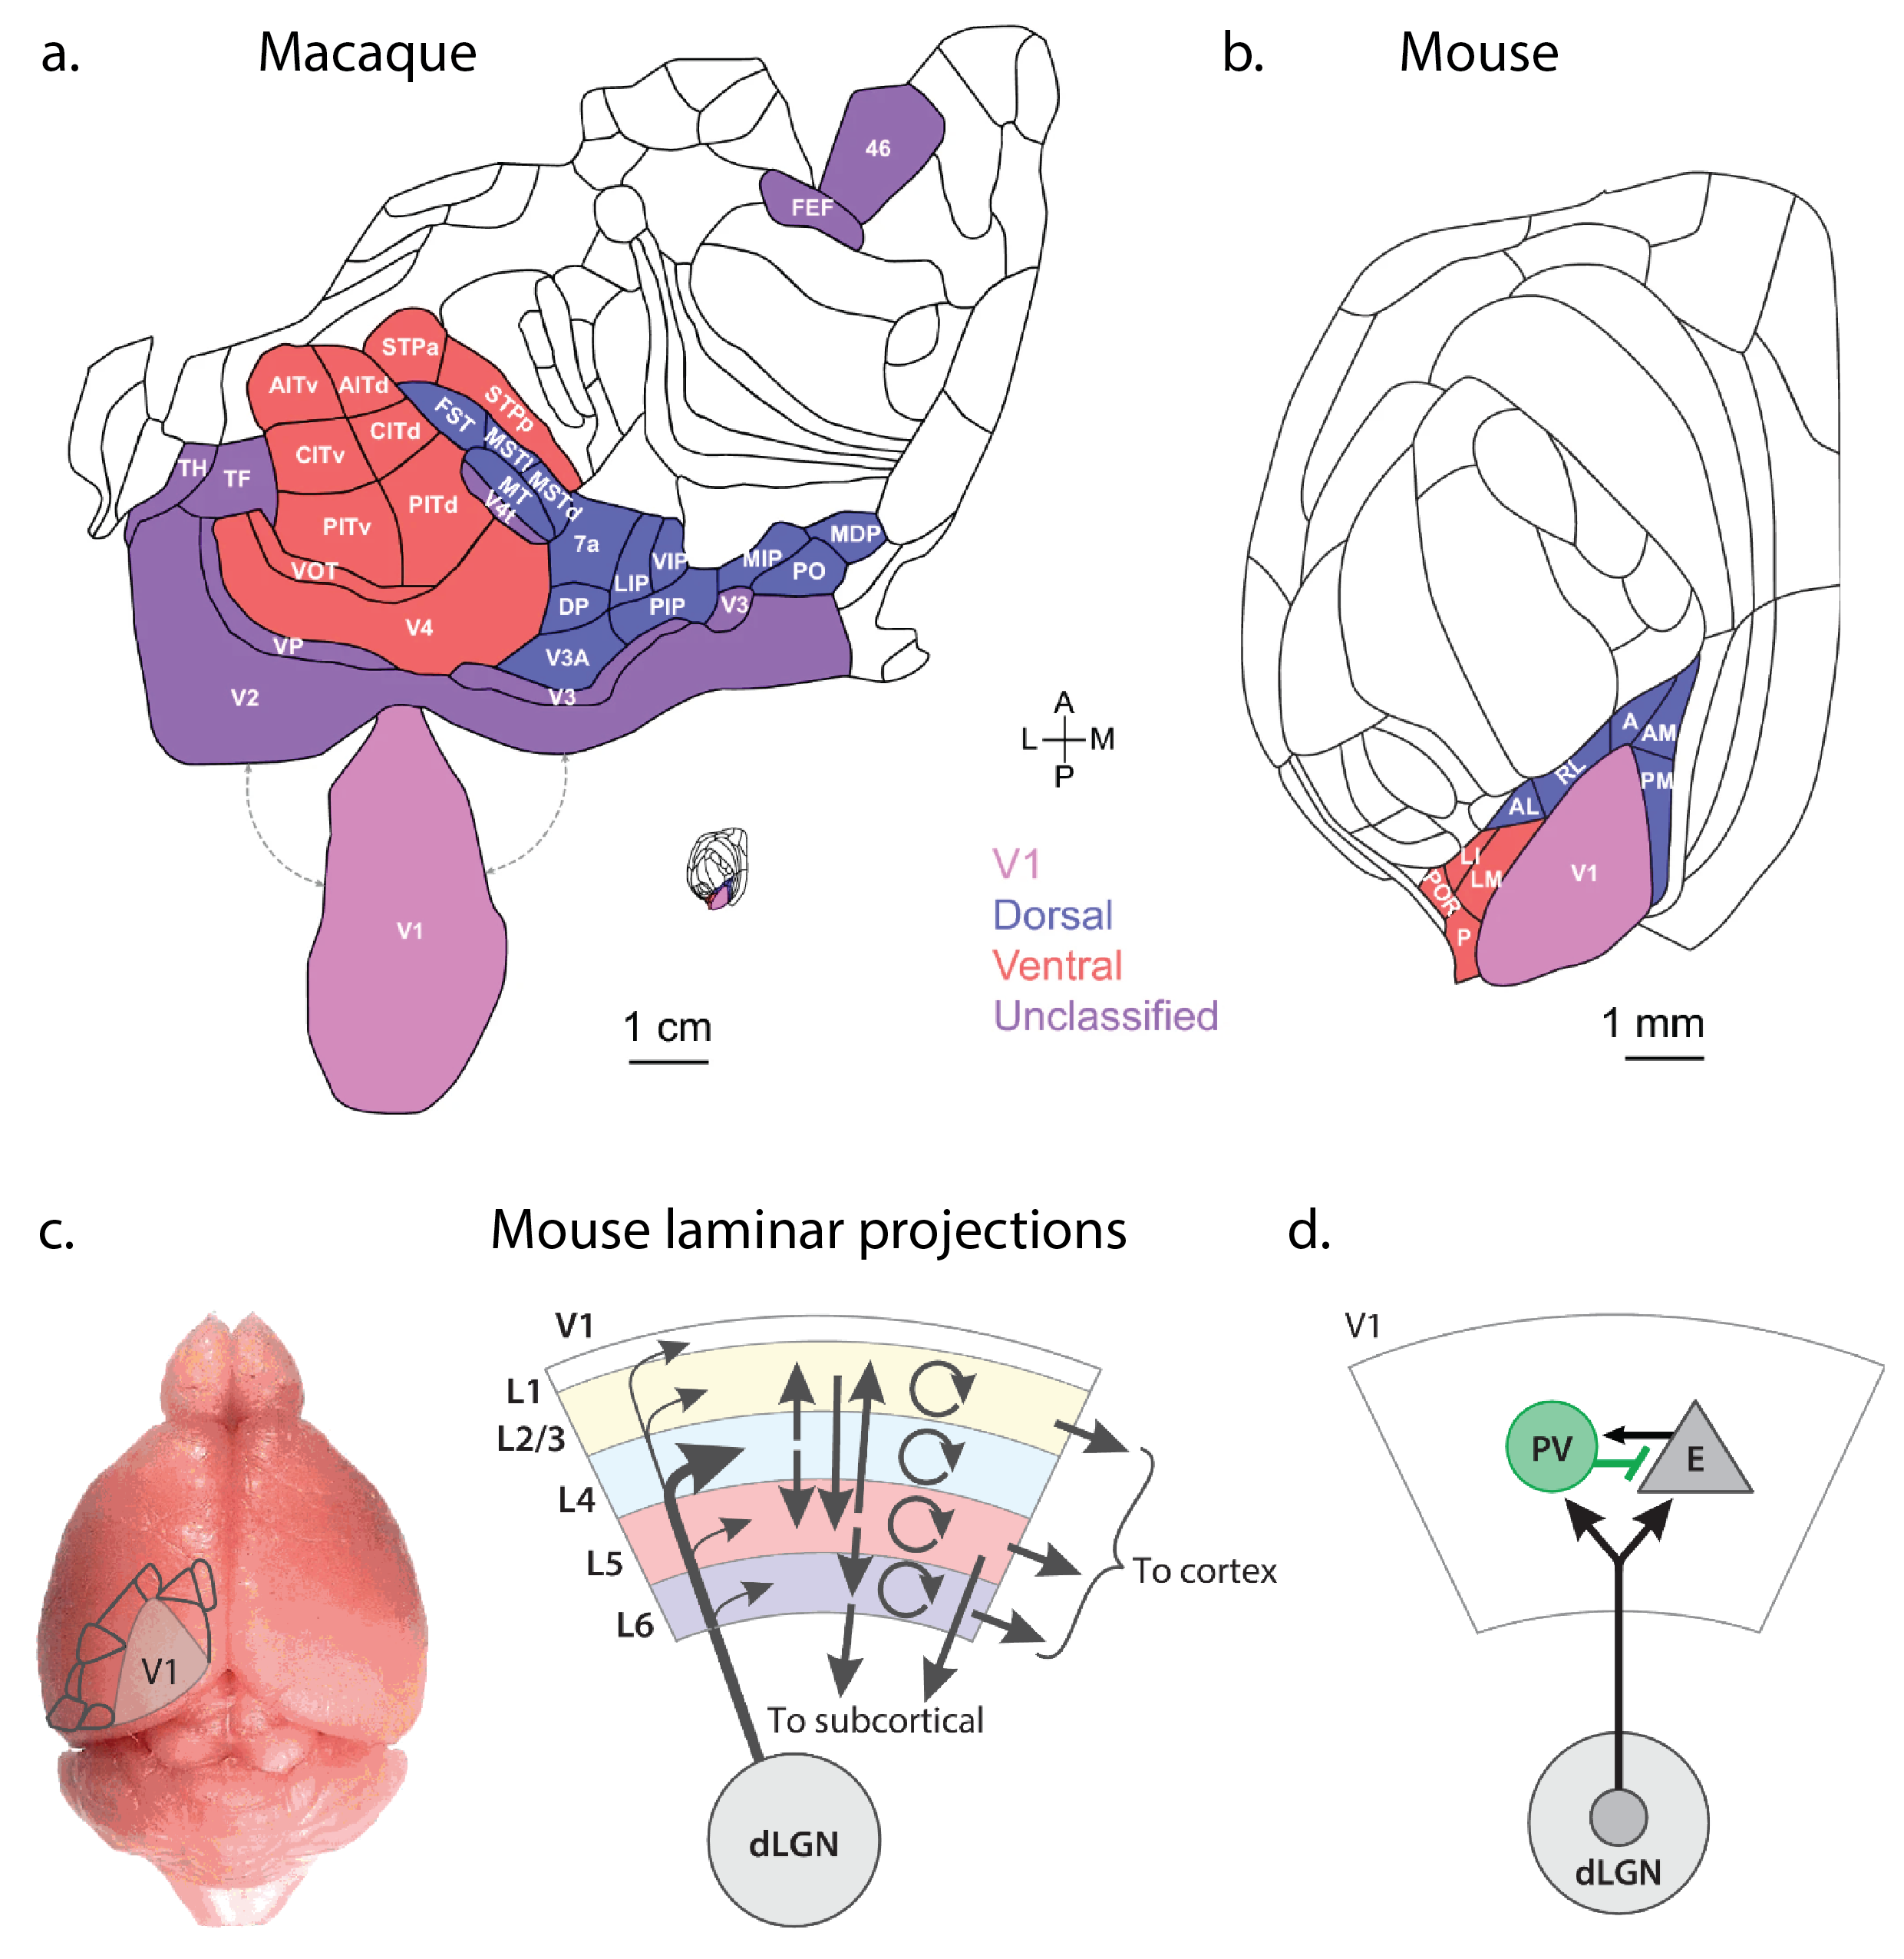
\includegraphics[width=1.0 \textwidth]{adjusted_figures/Laminar_Figure.png}
  \caption{a. The visual system of the macaque, visualising the hierarchical difference with the mouse visual system \autocite{gamanutAnatomicalFunctionalConnectomes2022}. b. The mouse visual system, highlighting the dorsal and the ventral stream, specifically ventral area LM as a potential homologue for macaque V2. c. The visual system mapped on a cortical image and a description of the laminar projections within V1. Similar to the organisation in the macaque, input from the dLGN is predominantly projected to layer 4, which projects to L2/3 and L5. d. Feedforward input mainly targets excitatory pyramidal cells and PV inhibitory interneurons, indicating that these cells might be of importance for the integration of feedforward and feedback signals.
  \autocite{niellHowCorticalCircuits2021}}
  \label{fig:Laminar_Figure}
\end{figure}


% Simple models orientation selectivity and  models for recurrent boundary completion (Grossberg), and deep learning models?

% Orientation selectivity is different in mouse vs primate so talk about models
%- models:
% Hubel DH, Wiesel TN (1962) Receptive fields, binocular interaction and functional architecture in the cat’s visual cortex. J Physiol 160:106–154. Medline
% Nguyen, Freeman 2019, model Hebbian strengthening spatially offset.
% Priebe 2016, Annual review Mechanisms of Orientation selectivity in V1

% - physiology
% Scholl, Corey, Priebe 2013, emergence orientation selectivity mammalian visual pathway
% Niell and Stryker 2008, ighly selective receptive fields in mouse visual cortex 
%- filling in 
% Filling-In the Forms: Surface and Boundary Interactions in Visual cortex
% Mechanism of surface completion: Perceptual Filling-In of texture Spillman De Weerd
%\subsection{Orientation selectivity in the visual system.}
To accurately represent an illusory contour, the visual system must be sensitive to the local orientation of the horizontal inducer lines to effectively determine the global spatial relationship between them. V1 is the first visual area where cells sensitive for orientation are found. Both retinal ganglion cells and their target LGN relay cells have circularly symmetric receptive fields and respond to nearly any stimulus within these fields. V1 neurons, however, are responsive to a number of stimulus attributes, such as orientation, motion direction, size, and binocular disparity of visual contours \autocite{hubelReceptiveFieldsBinocular1962}. 
Early models proposed by \textcite{hubelReceptiveFieldsBinocular1962} emphasised the convergence of signals from the dLGN to V1, suggesting a hierarchical integration of visual information. Physiologically V1 neurons can be described as simple or complex cells and are both orientation selective \autocite{skottunClassifyingSimpleComplex1991}. Simple cells receive direct input from the dLGN relay cells and their receptive field responses are characterised by segregated ON and OFF fields that prefer light or dark input, respectively. These subfields are elongated taking on an elliptical shape along the axis of the neuron's preferred orientation \hyperref[fig:LIF_Overview]{(figure 3a)}. Due to the segregated ON and OFF subfields their responses are sensitive to changes in phase and polarity \autocite{mechlerClassificationSimpleComplex2002}. 
\bigbreak
In contrast, complex cells that receive input from V1 simple cells have receptive fields in which ON and OFF regions are not spatially segregated. Therefore, complex cells respond to both increases and decreases in luminance at the same location and are not sensitive to stimulus polarity or tuned to a particular phase. An important question is how the spatial offset of ON and OFF subfields are developed, since these pathways are not segregated within the LGN. \textcite{nguyenModelOriginDevelopment2019} demonstrated that through a process of Hebbian learning the ON and OFF inputs could be sufficiently segregated to produce orientation selective neurons. In their simulations they simulated a 6 x 6 degree patch of visual field and divide that patch with random ON and OFF channels. Then they stimulated neuronal responses using a drifting grating over the full range of orientations. Each cycle in the development process then consisted of increasing the weights of all synapses for one randomly chosen subcortical channel. If the firing rate of a cortical neuron increased as a result, the synapse between the channel and the cortical target remained strengthened, and was otherwise decreased. After roughly 16000 cycles they found segregated ON and OFF subfields that was sufficient for orientation tuning. Still, the question remains whether a strict feedforward process is also sufficient for orientation tuning in physiology.
\bigbreak
To test whether orientation selectivity is a strict thalamocortical feedforward process or that these functional properties are a product of neuronal mechanisms on the cortical level \textcite{fersterOrientationSelectivityThalamic1996} inhibited cortical spiking and measured sub-threshold responses. They found that V1 neuron orientation selectivity is largely unaffected by cortical inactivation, providing evidence that the feedforward information transmitted by the LGN relay cells are sufficient to be transformed into orientation selective responses and that cortical circuitry is not required to refine these responses. Despite evidence showing similarities between mammals for how orientation selectivity originates, there are also large differences in the functional organisation across species. For instance, neurons in mouse V1 are not organised in columns with similar orientation preferences, as in primates. Mice also do not have the same pattern of functional segregation by layer that primates exhibit in which simple cells are found more in L4 and complex cells in deeper L2/3 \autocite{martinezReceptiveFieldStructure2005}. Instead, in the mouse, simple and complex cells are evenly distributed across cortical layers \autocite{niellHighlySelectiveReceptive2008}. Nevertheless, these differences in functional organisation are demonstrated to have a minimal impact on the functional properties of orientation tuning \autocite{hooserOrientationSelectivityOrientation2005}. Understanding the neuronal mechanisms of orientation selectivity across species is fundamental to the goal of understanding more complex perceptual phenomena, such as the perception of illusory contours. This leads us into an examination of various models that attempt to explain how the visual system integrates local and global information to have a shape or contour emerge from inducer shapes.    

%\subsection{Computational models for illusory contour representation.}
% Challenging deep learning models with abutting grating. Need for recurrency.

% A widespread view is that most texture segregation can be accounted for by differences in the spatial frequency content of texture regions, simple cells. Evidence from both psychophysical and physiological studies indicate, however, that beyond these early filtering stages, there are stages of 3-D boundary segmentation and surface representation that are used to segregate textures. \autocite{grossbergTextureSegregationSurface1998} (endstopped cells?)
% They arrive at a
% mutually consistent representation through reciprocal
% interactions. These interactions have been interpreted in
% terms of pathways joining the interblob and blob cortical streams between cortical areas V1 and V4 [19]. They
% are here used to explain texture segregation data for
% which early filtering mechanisms are insufficient. (Reciprocal, recurrency)
% endstopped cells for local detection
% bipole AND gate, however are orthogonally tuned, should not be local then larger receptive field HVAs
% biep.
\bigbreak
A recent study by \textcite{fanChallengingDeepLearning2023} explores the challenges deep neural networks (DNNs) face in representing illusory contours, specifically through the abutting grating illusion. Illusory contours, such as those seen in the abutting grating illusion, evoke perceptions of boundaries where none exist, a phenomenon that standard edge detectors cannot handle. The study highlights the failure of convolutional neural networks (CNNs) in revealing activity along these contours and proposes that recurrent processing, akin to that in biological vision, is crucial for accurate representation. In biological systems, recurrent connections allow for the integration of contextual information, essential for resolving ambiguities and ensuring consistent perceptual grouping and boundary completion. DNNs, which lack such recurrency, often fail in tasks involving illusory contours, underscoring a significant gap between artificial and biological vision systems \autocite{fanChallengingDeepLearning2023}.
\bigbreak
Grossberg, Mingolla, Peterhans, and von der Heydt have significantly contributed to understanding the neural mechanisms behind boundary completion and figure-ground separation. Their models incorporate endstopping and bipole cells to simulate how the brain perceives continuous boundaries from fragmented visual information. Grossberg and Mingolla's neural dynamics model, for instance, explains how visual inputs activate the Boundary Contour System (BCS), which interacts with the Feature Contour System (FCS) through feedback loops to complete boundaries and surfaces. This interaction is critical for the perception of illusory contours and shapes \autocite{grossbergTextureSegregationSurface1998}. Peterhans and von der Heydt expanded on these ideas by demonstrating that endstopped cells in the visual cortex, particularly in V1 and V2 areas, respond to lines and edges, contributing to the perception of illusory contours through mechanisms that integrate local orientation signals into coherent shapes\autocite{grossbergTextureSegregationSurface1998}. These endstopped neurons are maximally activated when lines or edges terminate within their receptive field but deactivate when the lines extend through it, making them crucial for detecting terminations and corners, fundamental elements in creating the perception of contours. Grossberg highlights the need for another cell type, the bipole cell. Bipole cells are senstive to collinear alignment of edges in local boundary detection, they are capable of integrating endstopped cells and can be used to complete open boundaries. Higher visual areas such as V2 and V4 are necessary for integrating information over larger spatial extents and bridging gaps between endstopped points. These areas use feedback connections to complex cells in earlier visual areas, reinforcing and refining the initial boundary signals to create stable and coherent perceptions of illusory contours.
\bigbreak
In conclusion, while bipole cells and endstopped neurons play crucial roles in local boundary detection, the full representation of illusory contours requires a more integrated approach involving higher visual areas and recurrent processing. This hierarchical and recursive processing framework enables the visual system to perceive complex shapes and contours that are not explicitly present in the visual input, a sophistication that current DNNs lack. Thus, integrating recurrent connections and feedback mechanisms in artificial vision systems is essential for advancing their capability to mimic primate and mice cortical architectures \autocite{grossbergHowVisualIllusions2014,grossbergTextureSegregationSurface1998}. 
\bigbreak
%\subsection{Current study local circuit structure for recurrent filling in.}
The abutting grating and Kanizsa illusions are both characterised by congruent illusory inducing points, identifiable by the presence of aligned line endings. Kanizsa inducers are considered more complex than abutting line inducers because each inducer point forms part of a corner, essentially two line ends meeting at an angle. In contrast, the abutting grating illusion is simpler, with its inducer points as single-line ends and, therefore, could be represented by a single endstopped cell \hyperref[fig:figure_1]{(figure 1c)}.
Nonetheless, cells sensitive to length might be fundamental to encoding both illusions, known as endstopped cells. Initially classified by Hubel and Wiesel in the cat's primary visual cortex (V1) in 1969, these cells are orientation-tuned and exhibit inhibition when a line segment exceeds their excitatory receptive field, leading to their initial characterisation as hypercomplex cells for their complex cell properties, such as stimulus polarity invariance, combined with inhibitory end zones \autocite{hubelRECEPTIVEFIELDSFUNCTIONAL1965}. Subsequent research revealed that a significant portion of V1 neurons exhibit endstopping to varying degrees across different species, including primates, cats, and mice \autocite{deangelisLengthWidthTuning1994,jonesSurroundSuppressionPrimate2001,sceniakVisualSpatialCharacterization2001}. Moreover, computational models have shown that endstopping can sufficiently delineate figures from the background and reconstruct illusory contours \autocite{vonderheydtMechanismsContourPerception1989}, suggesting that endstopped cell integration might serve as a universal neural mechanism for segmenting the visual field and to generating illusory contours.

%ToDo add a section of how endstopping is not caused by direct inhibitory endzones: \autocite{sillitoContributionExcitatoryInhibitory1977}
% Part under here is wrongly cited, has to be worked out again:
\bigbreak
Despite these insights, neurophysiological studies have largely overlooked how endstopping is integrated into higher visual areas for illusory contour perception. Previous computational simulations, while informative, have relied on feed-forward convolutions without accounting for biological constraints, such as direct inhibition to simulate negative end zones \autocite{sillitoContributionExcitatoryInhibitory1977}, and have not incorporated feedback mechanisms now recognised as crucial for the representation of illusory contours in lower visual areas. Addressing this gap, our current research endeavours to simulate endstopping using leaky integrate and fire (LIF) neurons and to integrate endstopped microcircuits through population rate models to accurately represent the abutting grating illusion. Our findings shed light on the minimal microcircuit necessary to exhibit end-stop characteristics, further illuminating how the representation of illusory contours through recurrent activity is modulated by the orientation selectivity of endstopped cells in higher visual areas. By incorporating endstopped cells into a hierarchical model, we aim to elucidate the neural mechanisms underlying illusory contour perception and to provide a comprehensive understanding of how the visual system processes illusory contours.
\bigbreak
This study investigates whether endstopping in V1 can occur solely through feedforward signals without direct inhibition or if a feedback mechanism is essential for activating inhibitory end zones. By simulating the representation of the abutting grating illusion via endstopped cell-driven recurrent activity, we explore the physiological constraints on integrating orientation-tuned endstopped cells in higher visual areas. Our goal is to elucidate how endstopped cells contribute to the perception of illusory contours and their integration within the visual cortex hierarchy. We hypothesize that endstopped cells are crucial for the representation of illusory contours and that their orientation tuning is modulated by feedback signals from higher visual areas. Our results will provide insights into the neural mechanisms underlying illusory contour perception and the hierarchical processing of visual information in the mammalian visual system.


\newpage
\section*{Methods}
% Introduction that states that we used two models with a rationalisation of why
%\subsection{Point neuron model and population neuron model.}
To investigate the minimal circuit necessary for endstopping and its role in generating illusory contours within the visual cortex of the mouse, the current study used two distinct computational frameworks. In the initial phase of the investigation, the utilised LIF models allowed us to simulate the spatial and temporal integration of synaptic input, on the single-cell level. This approach provided a foundational circuitry for orientation selectivity, complex cell features such as polarity invariance, and endstopping or length tuning. However, the current connectivity between LIF cells was set manually, and the complexity and computational demands associated with the tuning of each neuron constrained the current study to shift towards population cell models for the subsequent phase. Moreover, this phase focused on the generation of illusory contour responses through feedforward and feedback interactions. Nevertheless, the LIF network allowed us to estimate the necessary number of cells and the connectivity between cells required to create a stable neural mechanism for endstopping. The population models could then abstract this behaviour into a computationally tractable form, enabling efficient simulation of illusory contour generation throughout the visual hierarchy. 
\\
%\subsection{Simulating the Local microcircuit for Endstopping.}
To create the network for generating endstopping behaviour, the Brain Modelling Toolkit (BMTK) was used to define and connect nodes. We initialised an instance of the NetworkBuilder class provided by BMTK to construct an architecture of spiking point neurons, creating networks for both the dorsal lateral geniculate nucleus (dLGN) and the primary visual cortex (V1). Then visual stimuli were dynamically presented through a three-dimensional array format (t, y, x), with each entry along the first dimension (time, t) representing a frame, and input organised along the vertical (y) and horizontal (x) dimensions. The BMTK simulation pipeline processed visual information through a series of steps reflecting the increase in neural complexity of the visual system. This toolkit's flexibility allowed for precise control over the spatial arrangement and connectivity of neurons, facilitating the modelling of user specified neural circuits and their functional behaviours. \\
An important aspect of the BMTK is it segregation of the visual field as input and neural space. The BMTK has an input network called Filternet that generates firing rates based on information in the visual field. This effectively simulates the transformation from light intensity to neural signals as is done by the retina in visual system. Furthermore, the filter cells used in Filternet are responsive to either black or white light intensities thereby simulating the filtering properties of the dLGN, serving as spiking input to the cortex. This simulation environment allows for detailed analysis of how dLGN neurons process various visual inputs and contribute to the overall neural activity in V1. V1 was simulated via a simulator framework called Pointnet, which simulated point neuron networks with the NEST simulator. NEST is well-suited for modelling point neural networks and supports the integration of point-neuron models, making it ideal for simulating detailed spiking activity and synaptic interactions within the V1 network. Using Pointnet, we leveraged NEST's capabilities to simulate the complex dynamics of V1 neurons, including their interactions and resultant network behaviour. This approach enabled the modelling of cortical processing of visual information, where the integration of inputs from the dLGN and the intrinsic cortical circuitry results in the emergence of visual features such as orientation selectivity \hyperref[fig:LIF_Overview]{(Figure 3a)}, phase invariance\hyperref[fig:LIF_Overview]{(Figure 3a)}, and length tuning \hyperref[fig:LIF_Overview]{(Figure 3c)}. By separating the simulations into Filternet for the dLGN and Pointnet for the V1 cortex, we had great control over the thalamocortical transformation required for orientation selectivity, and guarantee the analysis at the appropriate level of detail.
\bigbreak

% Overview figure
\begin{figure}[H]
  \centering
  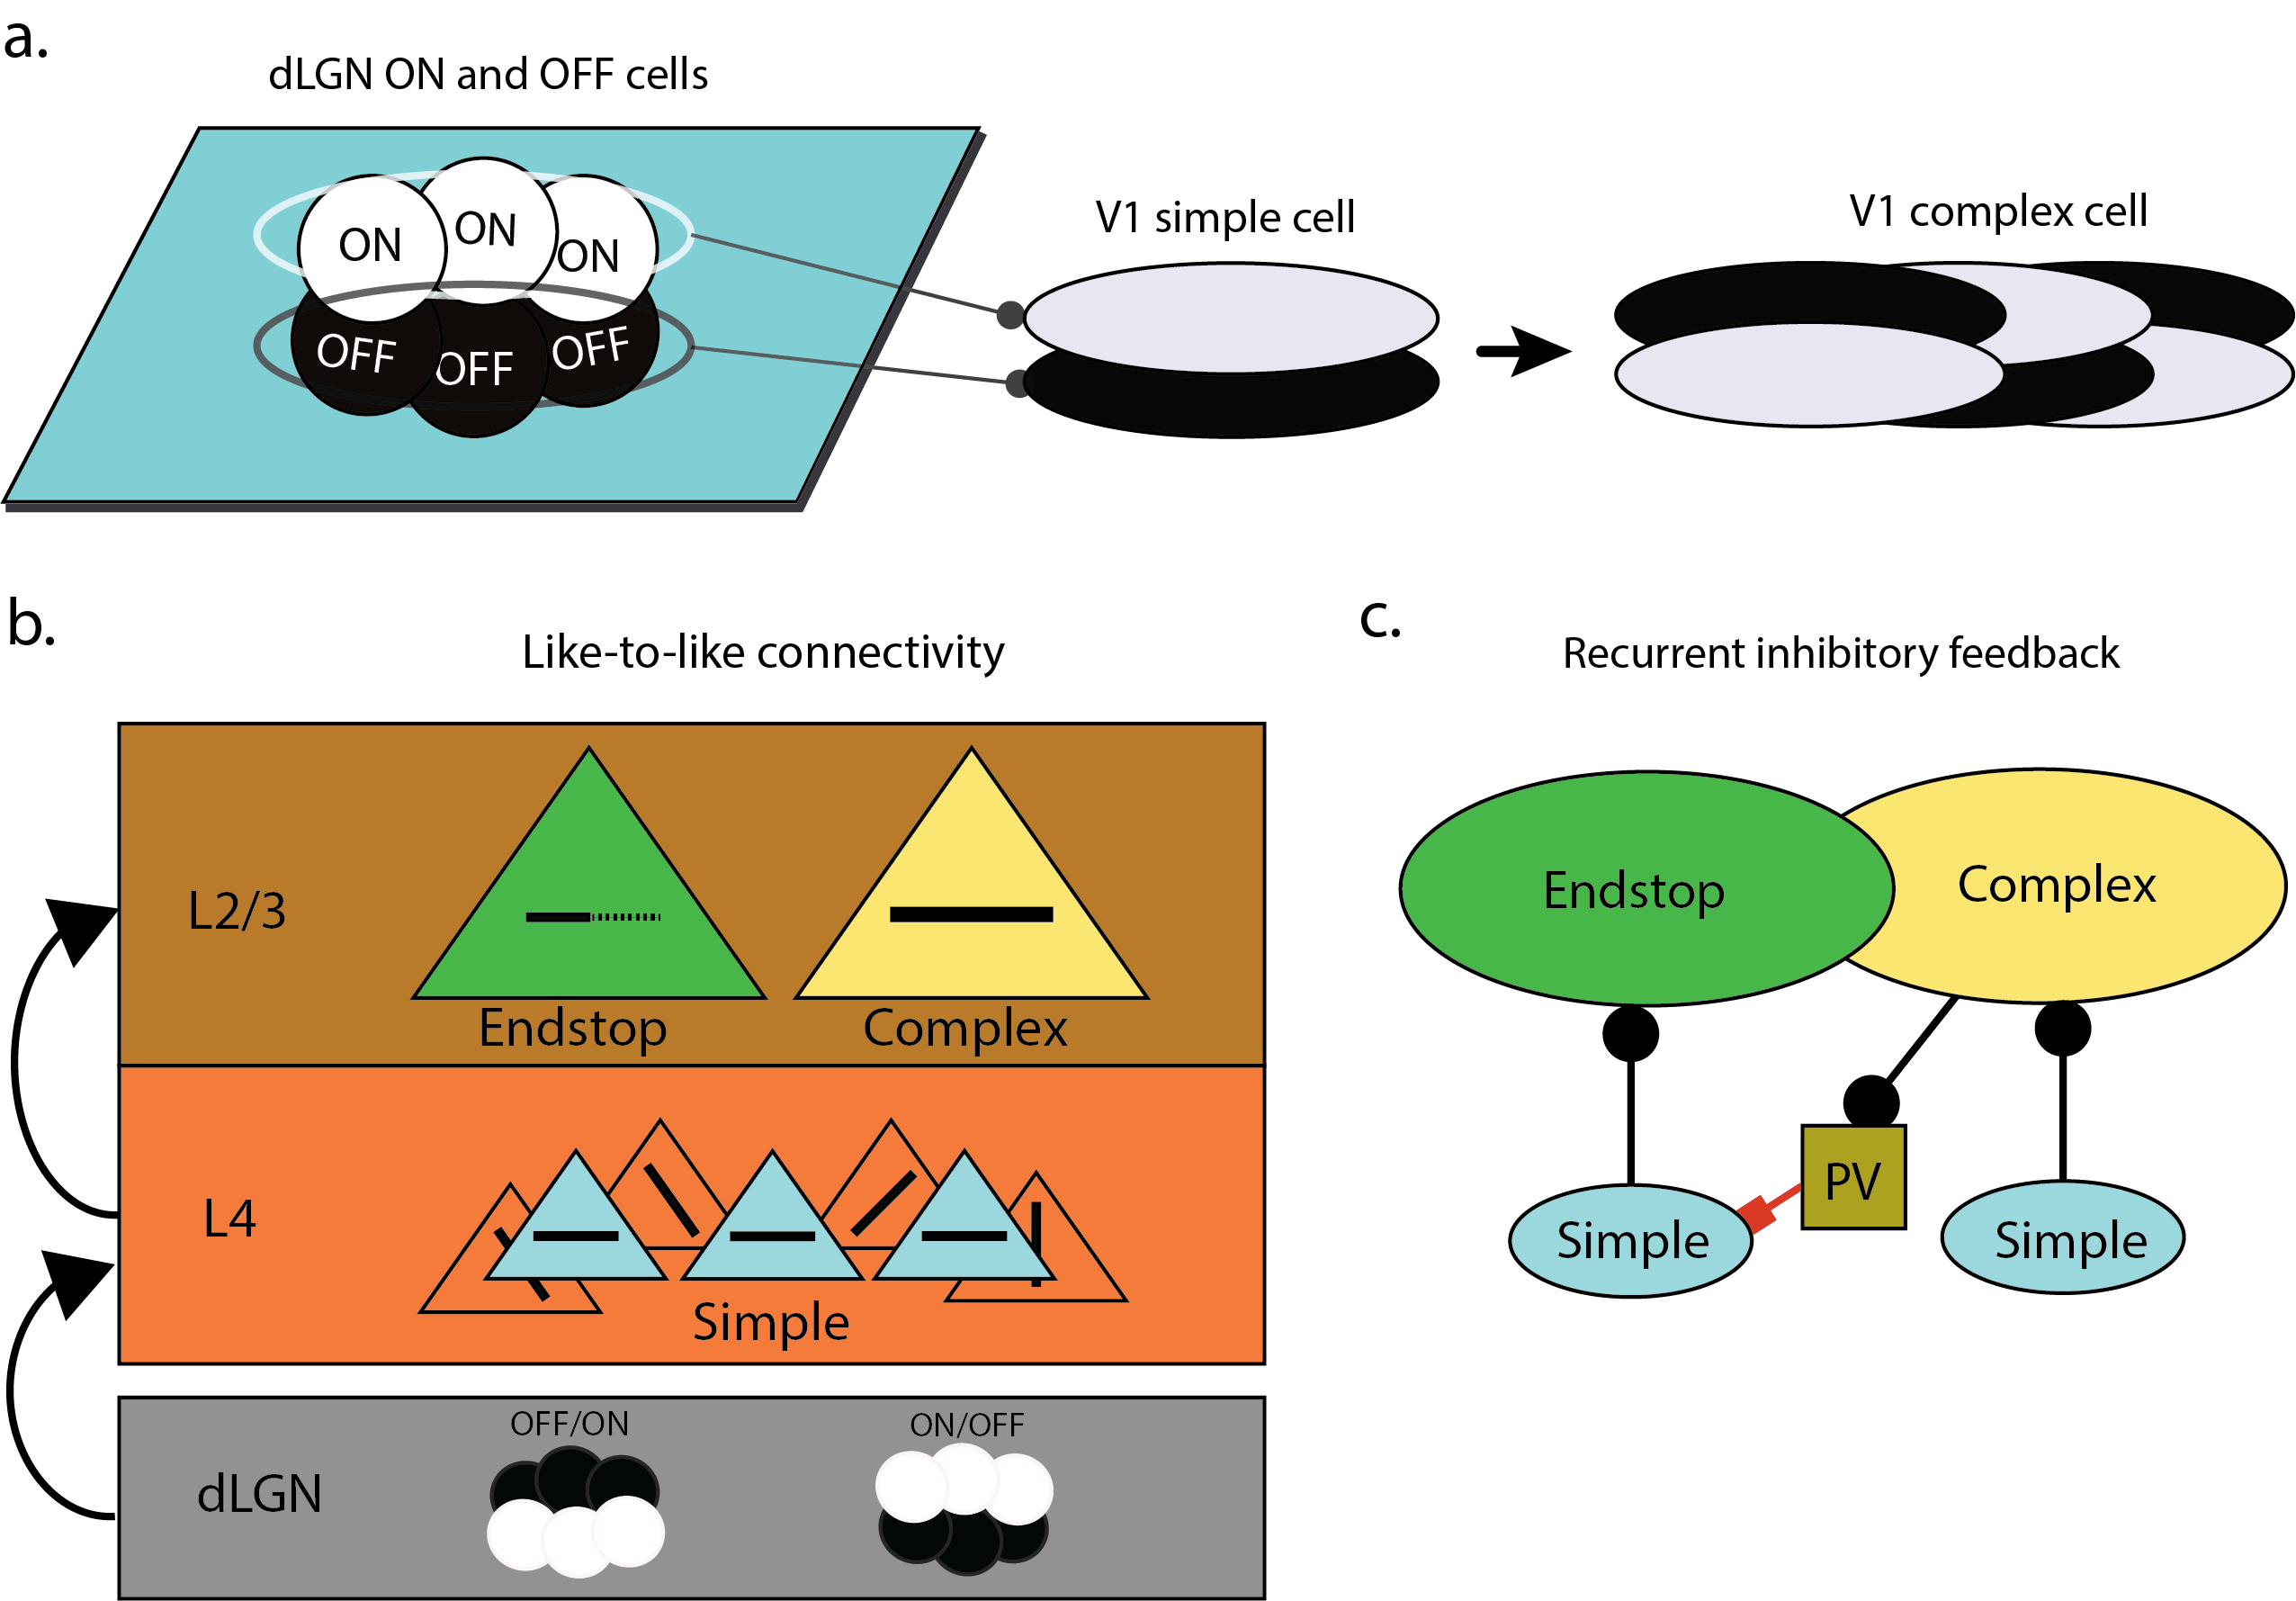
\includegraphics[width=1.0 \textwidth]{adjusted_figures/LIF_Overview_Receptive_Field_Methods.png}
  \caption{a. The dLGN ON and OFF cells that converge with a spatial offset onto a simple cell, creating a simple filter that responds to edges. Combining multiple simple cells with overlapping ON and OFF fields creates a complex cell. The complex cells, due to their overlapping subfields are not dependent on stimulus polarity and are phase invariant. b. A diagram showing the hierarchical complexity of cells that are connected based on their orientation tuning. The green endstopped cell is illustrated by a dotted line end, showing that an extended line end will result in a decreased firing rate. c. Shows how a particular endstopped microcircuit is made. Population of simple cells converge onto the endstopped and complex cell to give them feedforward input, however if a line would extend over the endstopped receptive field, stimulating the complex cell. A recurrent inhibitory feedback loop would inhibit the simple population that is responsible for the endstopped cell's drive and firing will decrease. }
  \label{fig:LIF_Overview}
\end{figure}

% ToDo: make sure no redundant information is in it. 
%\subsection{dLGN transformes light intensity to neural activity.}
The first relay station in the visual pathway is the dLGN, which receives input from the retina and transmits visual information to V1 for further processing. The dLGN processes visual stimuli through two distinct pathways: the ON and OFF pathways, which respond to increases and decreases in light intensity, respectively. These pathways are essential for encoding contrast and edge information in visual scenes, providing the initial processing steps that shape the neural representation of visual stimuli. By presenting visual stimuli to the dLGN network, we can effectively simulate the translation of light input into neural signals, creating the first layer for contrast detection in the visual system. Since we are interested in contrast, which is encoded in V1 rather than colour, only monochromatic greyscale stimuli were shown. To transform this input array into neural signals, the dLGN was simulated as a linear-non-linear Poisson cascade model. First, visual input within the space of the receptive field of the dLGN cell is convolved with a linear filter. Then a nonlinear function is applied to the output of the previous linear filter, giving the neuron's instantaneous spike rate as its output. Finally, this firing rate generates spikes according to an inhomogeneous Poisson process \autocite{moskovitzComparisonDeepLearning2018}. The current dLGN model consists of two unit types, ON and OFF surround cells, optimised to closely mimic mammalian thalamic cells \autocite{billehSystematicIntegrationStructural2020}. The ON and OFF cells of the LGN converge on a layer of simple cells, effectively simulating layer 4 (L4) of V1 (Figure \ref{fig:LIF_connectivity}a). This dual pathway of ON/OFF cells is essential for the initial segregation of visual information, setting the stage for more complex edge detection and contrast processing within higher cortical areas. We analyzed spiking features in response to static images. Therefore, we focused on modeling ON and OFF cells to have a predominantly sustained responses (sON and sOFF). We used the model templates in our node configuration to implement these cells in our network. The parameters for these cells were set based on values derived from electrophysiological recordings from the mouse dLGN, as reported by \textcite{durandComparisonVisualResponse2016} and \textcite{billehSystematicIntegrationStructural2020}.

\begin{figure}[H]
  \centering
  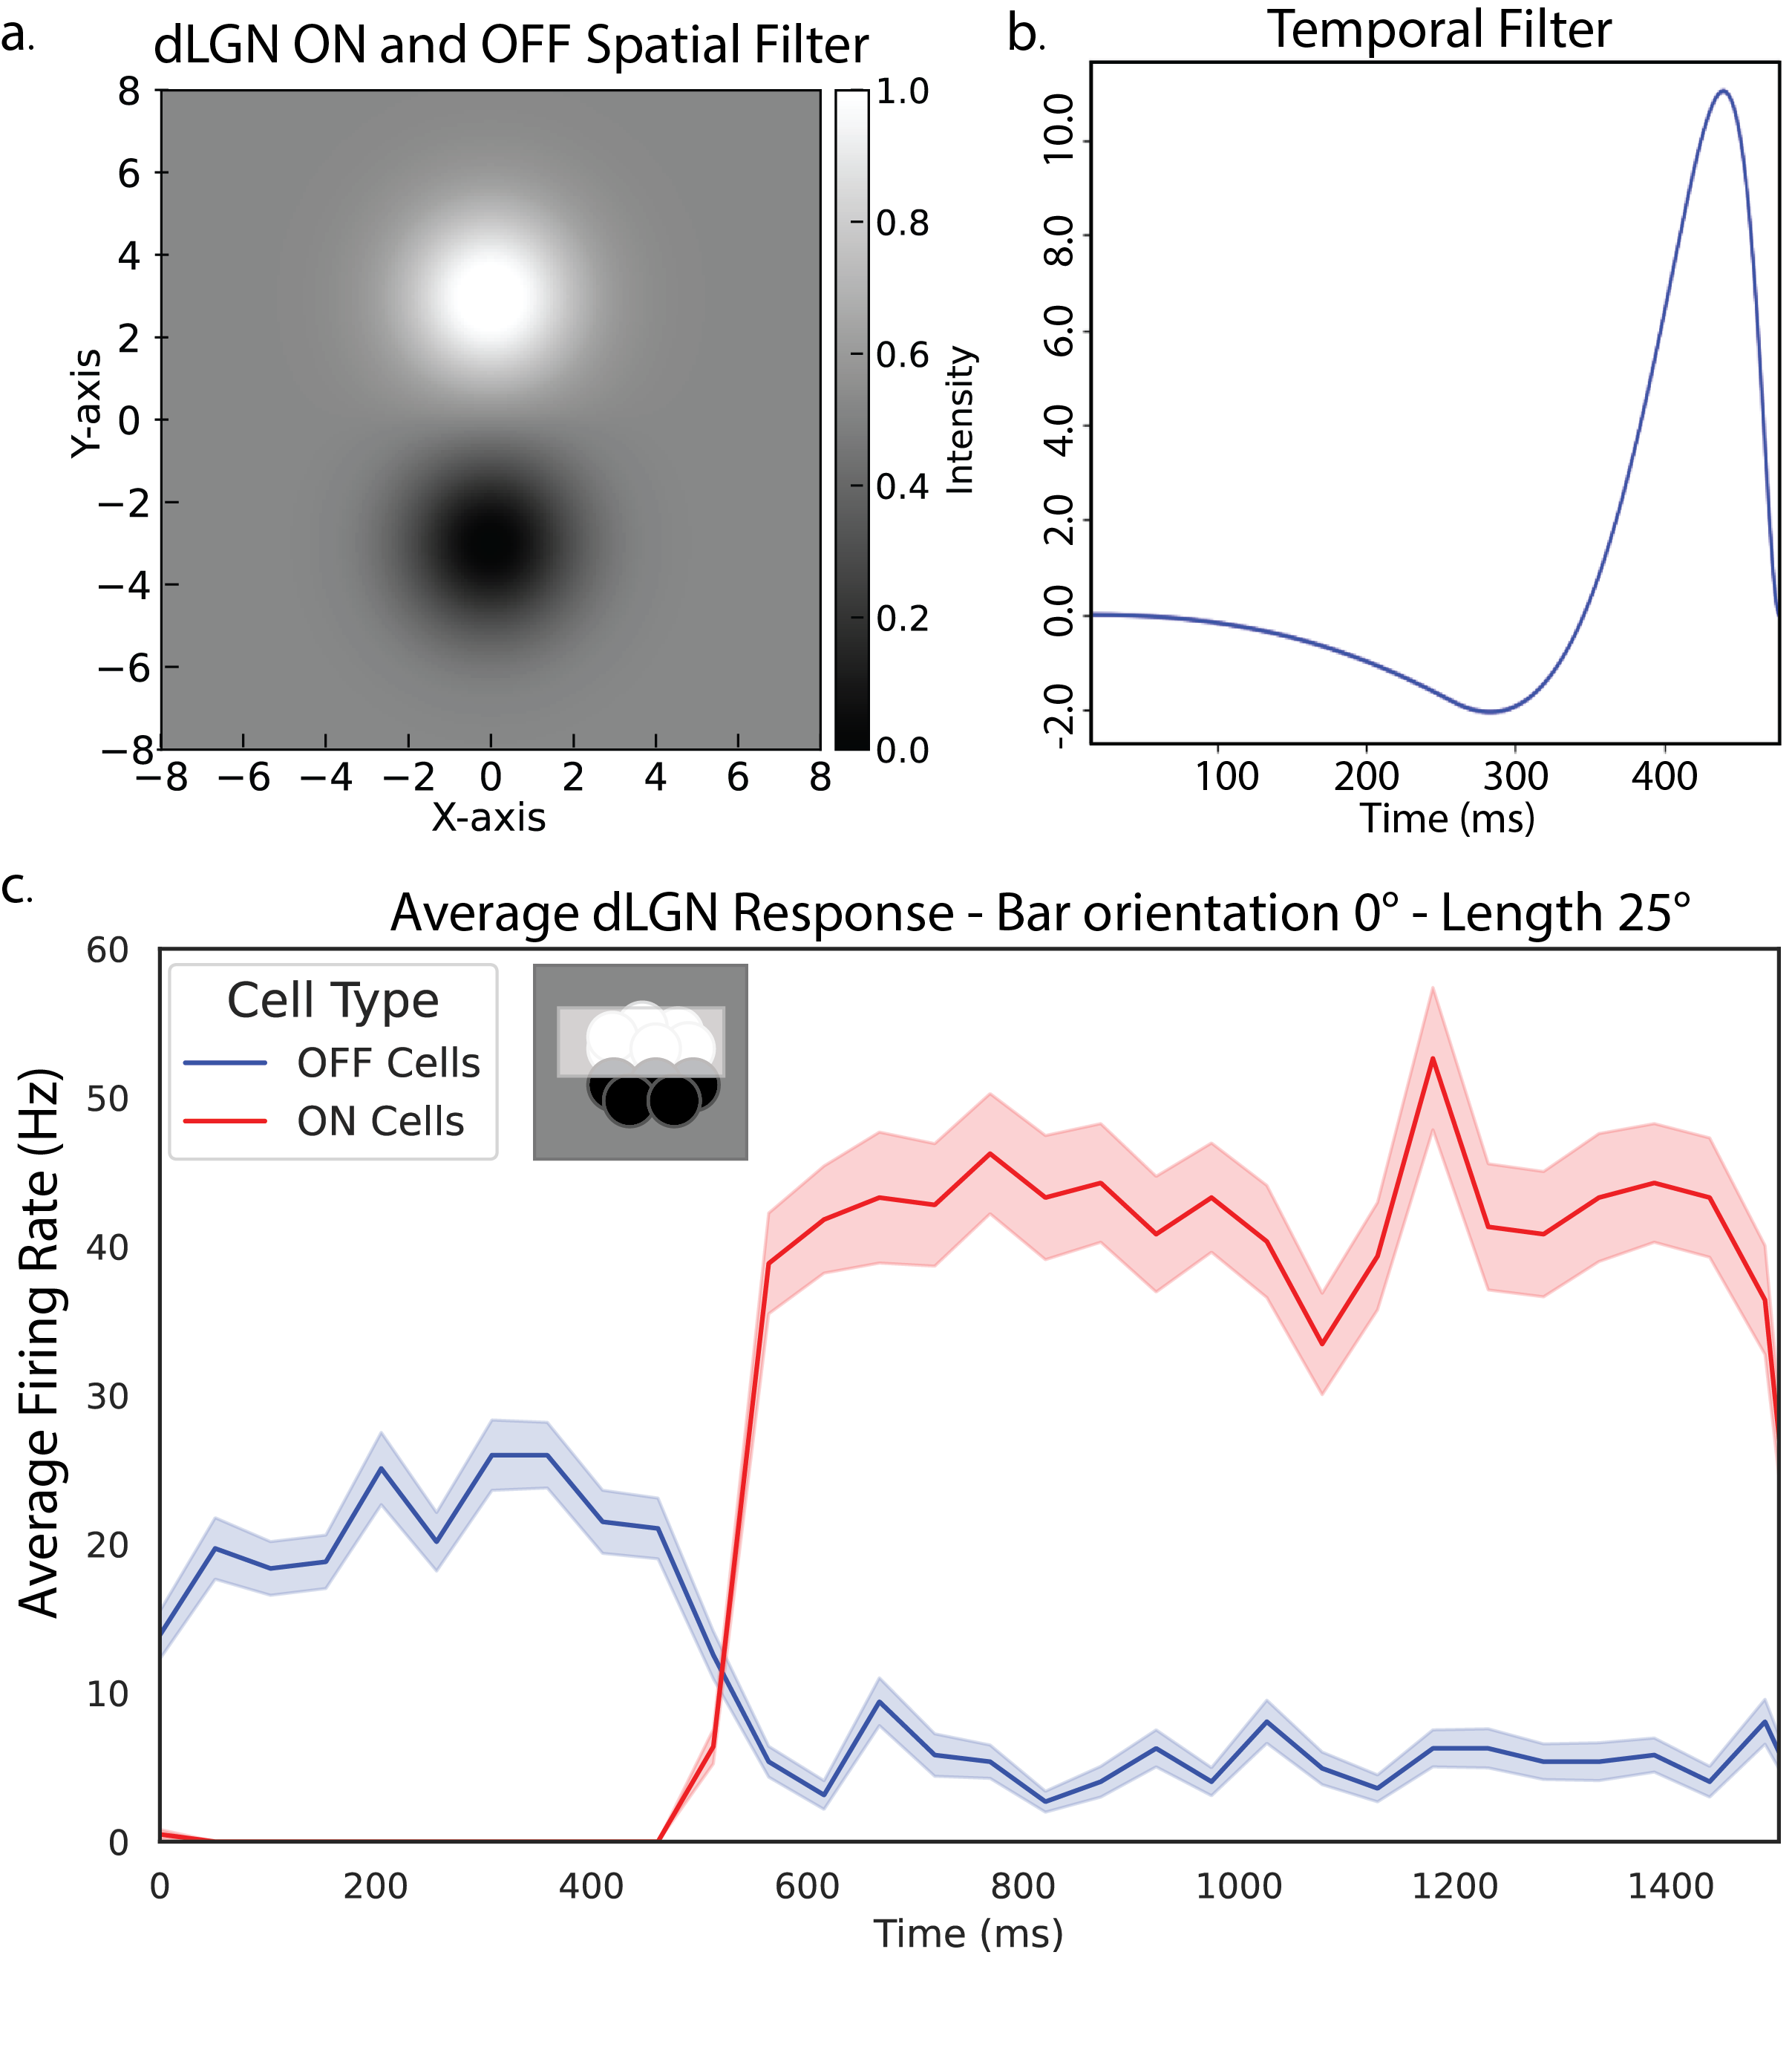
\includegraphics[width=1.0 \textwidth]{figures/lgn_response_fig.png}
  \caption{a. The ON and OFF spatial filters used as input to V1 simple cells. The ON and OFF filters are two inverted gaussian functions that are sensitive to bright and dark input, respectively. b. Each filter also has a temporal filter that dictates how the response changes through time. c. The ON and OFF response to a bar that is completely stimulating the ON cells as well as some minor stimulation to the OFF cells. The stimulus is a bar with a length of 25 visual degrees and is completely horizontal with a rotation of 0 degrees. All stimuli presented to the dLGN were monochromatic and could be represented by either ON or OFF cells.}
  \label{fig:LIF_connectivity}
\end{figure}

For the spatial filtering of the receptive fields, we employed a Gaussian filter characterised by its spatial size and rotation. The default spatial size was set to 5.0 spatial degrees for both rows and columns, which means the filter covered a 5-degree area in both the horizontal and vertical directions. The rotation of the filter was set to 0.0 degrees, indicating no rotation and ensuring alignment with the primary axes.

Temporal filtering was managed using a double cosine filter, which incorporates two cosine waves to model the time-dependent response of the neurons. This filter is defined by several key parameters: weights, k-peaks, and delays. The weight parameter controlled the amplitude of the two peaks in the cosine filter. The first peak had a higher amplitude (weights[0]) compared to the second peak (weights[1]). This reflects the biological observation that the initial response to a stimulus is typically stronger than subsequent responses. The k-peaks parameter determined the spread or width of the peaks. The first peak, associated with the initial response, had a narrower spread, while the second peak, representing the later response, had a broader spread. This setup ensures that the initial peak is sharp and quick, capturing rapid changes, whereas the second peak is more prolonged, capturing sustained responses.

The delay parameter controlled the timing of the peaks. The first delay (delays[0]) set the timing for the initial, larger peak, and the second delay (delays[1]) set the timing for the secondary, smaller peak. A smaller value for delays[0] resulted in a quicker initial response to changes in brightness, indicating that the neuron reacts promptly to the onset of a stimulus. Conversely, a larger value meant a slower initial response. Similarly, the value of delays[1] determined how quickly the secondary response occurred, with smaller values indicating quicker secondary responses and larger values indicating slower ones. By carefully configuring these parameters—weights for amplitude, k-peaks for spread, and delays for timing—we ensured that the dLGN cells accurately modelled the sustained neural responses to both ON and OFF inputs necessary for our study.

\begin{table}[H]
  \centering
  \caption{Parameters and Weights for LGN and V1 Cells}
  \begin{tabular}{lll}
  \toprule
  \textbf{Cell Type} & \textbf{Parameter} & \textbf{Description} \\
  \midrule
  \multirow{4}{*}{LGN} 
      & Optimized weight      & (7, -1) \\
      % & Parameter bounds   & P \\
      & Delays   & (0, 0) \\
      & K-peaks   & (30, 55) \\
  \midrule
  \multirow{7}{*}{V1} 
      & External current         & 0.0 nA \\
      & Membrane time constant        & 44.9 ms \\
      & Membrane capacitance          & 239.0 pF \\
      & Refractory period       & 3.0 ms \\
      & Resting potential          & -78.0 mV \\
      & Threshold potential         & -43.0 mV \\
      & Reset potential      & -55.0 mV \\
  \bottomrule
  \end{tabular}
\end{table}



% For the spatial filtering of the receptive fields, we employed a Gaussian filter characterised by its spatial size and rotation. The default spatial size was set to 5.0 spatial degrees for both rows and columns, with a rotation of 0.0 degrees. The temporal filtering was managed using a double cosine filter. The parameters for this filter included weights, kpeaks, and delays. The weight parameter controlled the amplitude of the two peaks in the cosine filter, with the first value being greater than the second (weights[0] > weights[1]). The kpeaks parameter determined the spread of the peaks, ensuring the second peak had a greater spread than the first.
% \bigbreak
% The delay parameter controlled the timing of the peaks, with delays[0] setting the delay for the first, larger peak and delays[1] setting the delay for the second, smaller peak. A smaller value for delays[0] resulted in a quicker initial response to brightness changes, while a larger value meant a slower initial response. Similarly, delays[1] determined how quickly the secondary response occurred, with smaller values indicating quicker secondary responses and larger values indicating slower ones. By carefully setting these parameters, we ensured that the LGN cells accurately modelled the sustained neural responses to both ON and OFF input necessary for our study.

% \begin{table}[H]
%   \centering
%   \caption{Parameters and Weights for LGN and V1 Cells}
%   \begin{tabular}{lll}
%   \toprule
%   \textbf{Cell Type} & \textbf{Parameter} & \textbf{Description} \\
%   \midrule
%   \multirow{4}{*}{LGN} 
%       & Optimized weight      & (7, -1) \\
%       % & Parameter bounds   & P \\
%       & Delays   & (0, 0) \\
%       & K-peaks   & (30, 55) \\
%   \midrule
%   \multirow{7}{*}{V1} 
%       & External current         & 0.0 nA \\
%       & Membrane time constant        & 44.9 ms \\
%       & Membrane capacitance          & 239.0 pF \\
%       & Refractory period       & 3.0 ms \\
%       & Resting potential          & -78.0 mV \\
%       & Threshold potential         & -43.0 mV \\
%       & Reset potential      & -55.0 mV \\
%   \bottomrule
%   \end{tabular}
% \end{table}
\bigbreak
%To Do rewrite more concise
%\subsection{Orientation Selectivity in V1}
To achieve orientation selectivity in V1 simple cells dLGN were strategically connected to form elliptical receptive fields. Specifically, we designed each simple cell in V1 to have a receptive field composed of two distinct elliptical regions: one for ON and one for OFF responses. These ellipses were positioned relative to each other and oriented along a specific angle, allowing the V1 cells to sample input selectively from ON and OFF LGN cells. To implement this, we first defined the receptive field for each V1 simple cell by setting the parameters of the ellipses. Each ellipse had a preferred orientation, which was determined by the angle of its major axis, reflecting the preferred orientation of the V1 cell. The separation between the centres of the ON and OFF ellipses was carefully specified to ensure that these regions were spatially distinct but aligned according to the desired orientation. This separation allowed the ON and OFF regions to be positioned, so they could selectively sample from the respective ON and OFF dLGN cells.

Connections from the dLGN cells to the V1 simple cells were established using a selective connection rule implemented through a connection function. This function determined whether an dLGN cell's position fell within the bounds of the ON or OFF ellipse of a given V1 cell. For each LGN cell, the function checked if the cell's position was within the elliptical boundary using a mathematical condition that defines whether a point lies inside an ellipse. This condition was based on the ellipse's centre, axes, and orientation, allowing precise determination of the inclusion of LGN cells within the receptive fields of the V1 cells. Once an LGN cell was identified as being within the receptive field of a V1 cell, synaptic connections were established with specific weights and delays. These synaptic parameters were carefully tuned to reflect the physiological properties of synaptic transmission observed in biological systems, such as a minimal refractory period of 2 ms. The synaptic weights determined the strength of the input from the LGN cell to the V1 cell, while the delays accounted for the time taken for the signal to travel between the two cells. The network construction involved creating a V1 network with simple cells characterised by their orientation, positions, and receptive field parameters, such as the separation between ellipses, the radius, and the aspect ratio of each ellipse. The positions of the V1 cells were generated within a specified spatial grid to simulate the realistic arrangement of neurons in the visual cortex. Similarly, the dLGN cells were distributed across a spatial grid with their positions randomly generated within defined bounds, reflecting the natural variability in the spatial distribution of these cells. The selective connection rule played a crucial role in achieving orientation selectivity. The rule iterated over all possible dLGN sources for each V1 target, checking for inclusion within the ellipses and establishing connections accordingly. This process ensured that each V1 simple cell received input from a specific subset of dLGN cells aligned with its receptive field configuration. By connecting each V1 cell to a well-defined set of ON and OFF LGN cells, the V1 cells could respond preferentially to specific orientations of visual stimuli. Through this method, elliptical receptive fields with distinct ON and OFF regions enabled the V1 simple cells to become orientation-selective. The careful design of the spatial arrangement of the ellipses, combined with the selective connection rules, ensured that the V1 cells exhibited orientation selectivity similar to that observed in biological visual systems. This approach provided a robust model for simulating orientation selectivity and the role of specific dLGN inputs in shaping the response properties of V1 neurons.

\begin{figure}[H]
    \centering
    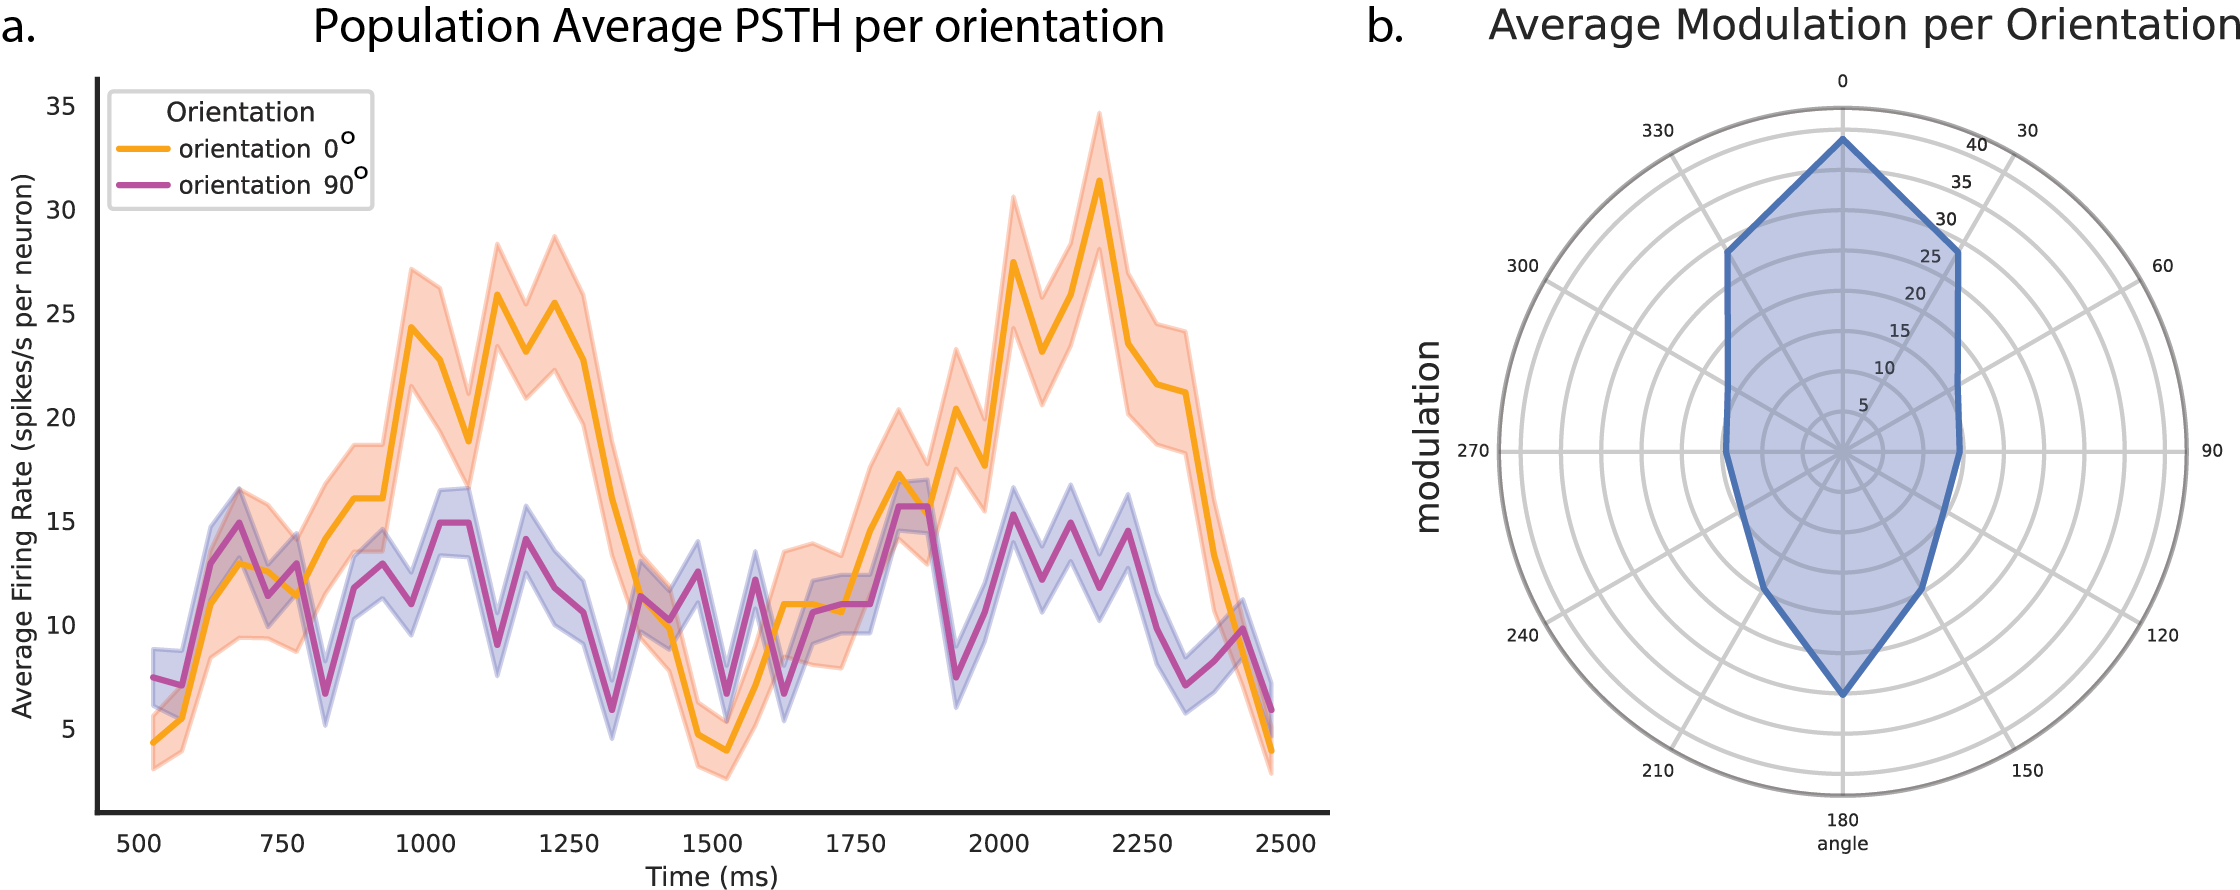
\includegraphics[width=1.0 \textwidth]{figures/figure_simple_orientation_tuning.png}
    \caption{a. The average orientation tuning of a population of simple cells. The input was a drifting grating with different orientations. In orange a horizontal drifting grating with 0 degrees rotation, and in purple a drifting grating with a 90 degree rotation. Simple cells show a phase sensitivity demonstrated by the two peaks, in which the cell receives no input from the dLGN. b. A polar plot showing the average firing modulation per orientation, showing that the cells respond to 0 and 180 degrees rotated stimuli.}
    \label{fig:simple cell orientation tuning}
\end{figure}

%\subsection{Polarity Invariance of Complex Cells.}
Subsequently, complex cells are created by strategically connecting these simple cells with each other. The process began by combining simple cells responsive to different phases (ON/OFF) to form complex cells; with the goal of creating a phase invariant complex cell. To create complex cells that respond to contours within their receptive field regardless of input polarity, a few retinotopically aligned simple cells were connected to achieve overlapping ON/OFF and OFF/ON receptive fields. The converging simple cells all had the same preferred orientation but different spatial phases creating a single complex cell \hyperref[fig:LIF_Overview]{(Figure 3b)}. The selective connection rule played a crucial role in this process. The rule iterated over all possible simple cell sources for each target complex cell, checking for alignment in orientation and differences in phase. Synaptic connections were established between the simple cells and the complex cell, ensuring that the complex cell received inputs from a diverse set of simple cells. This convergence allowed the complex cell to respond to a range of spatial phases of a given orientation, thereby achieving polarity invariance. To test whether our complex cells demonstrated polarity and phase invariance we presented the circuit with a drifting grating in the preferred orientation of the complex cell \hyperref[fig:polarity invariance]{figure 6b}. The drifting grating would in one spot of the visual field induce an alternating pattern between white and black. Therefore, ON/OFF cells and OFF/ON cells would also show an alternating peak in activity, whereas complex cells are expected to have a more stable firing pattern. In figure 6a the simple cell types clearly showed peaks at 30 Hz and decreasing to 0 Hz. In contrast, due to the converging simple cells, the complex cells have a stable activity above 30 Hz, also highlighted in the raster plots \hyperref[fig:polarity invariance]{figure 6c}. With these fundamental cell types with the addition of inhibitory interneurons it is possible to create endstopped length tuned cells. 

\begin{figure}[H]
    \centering
    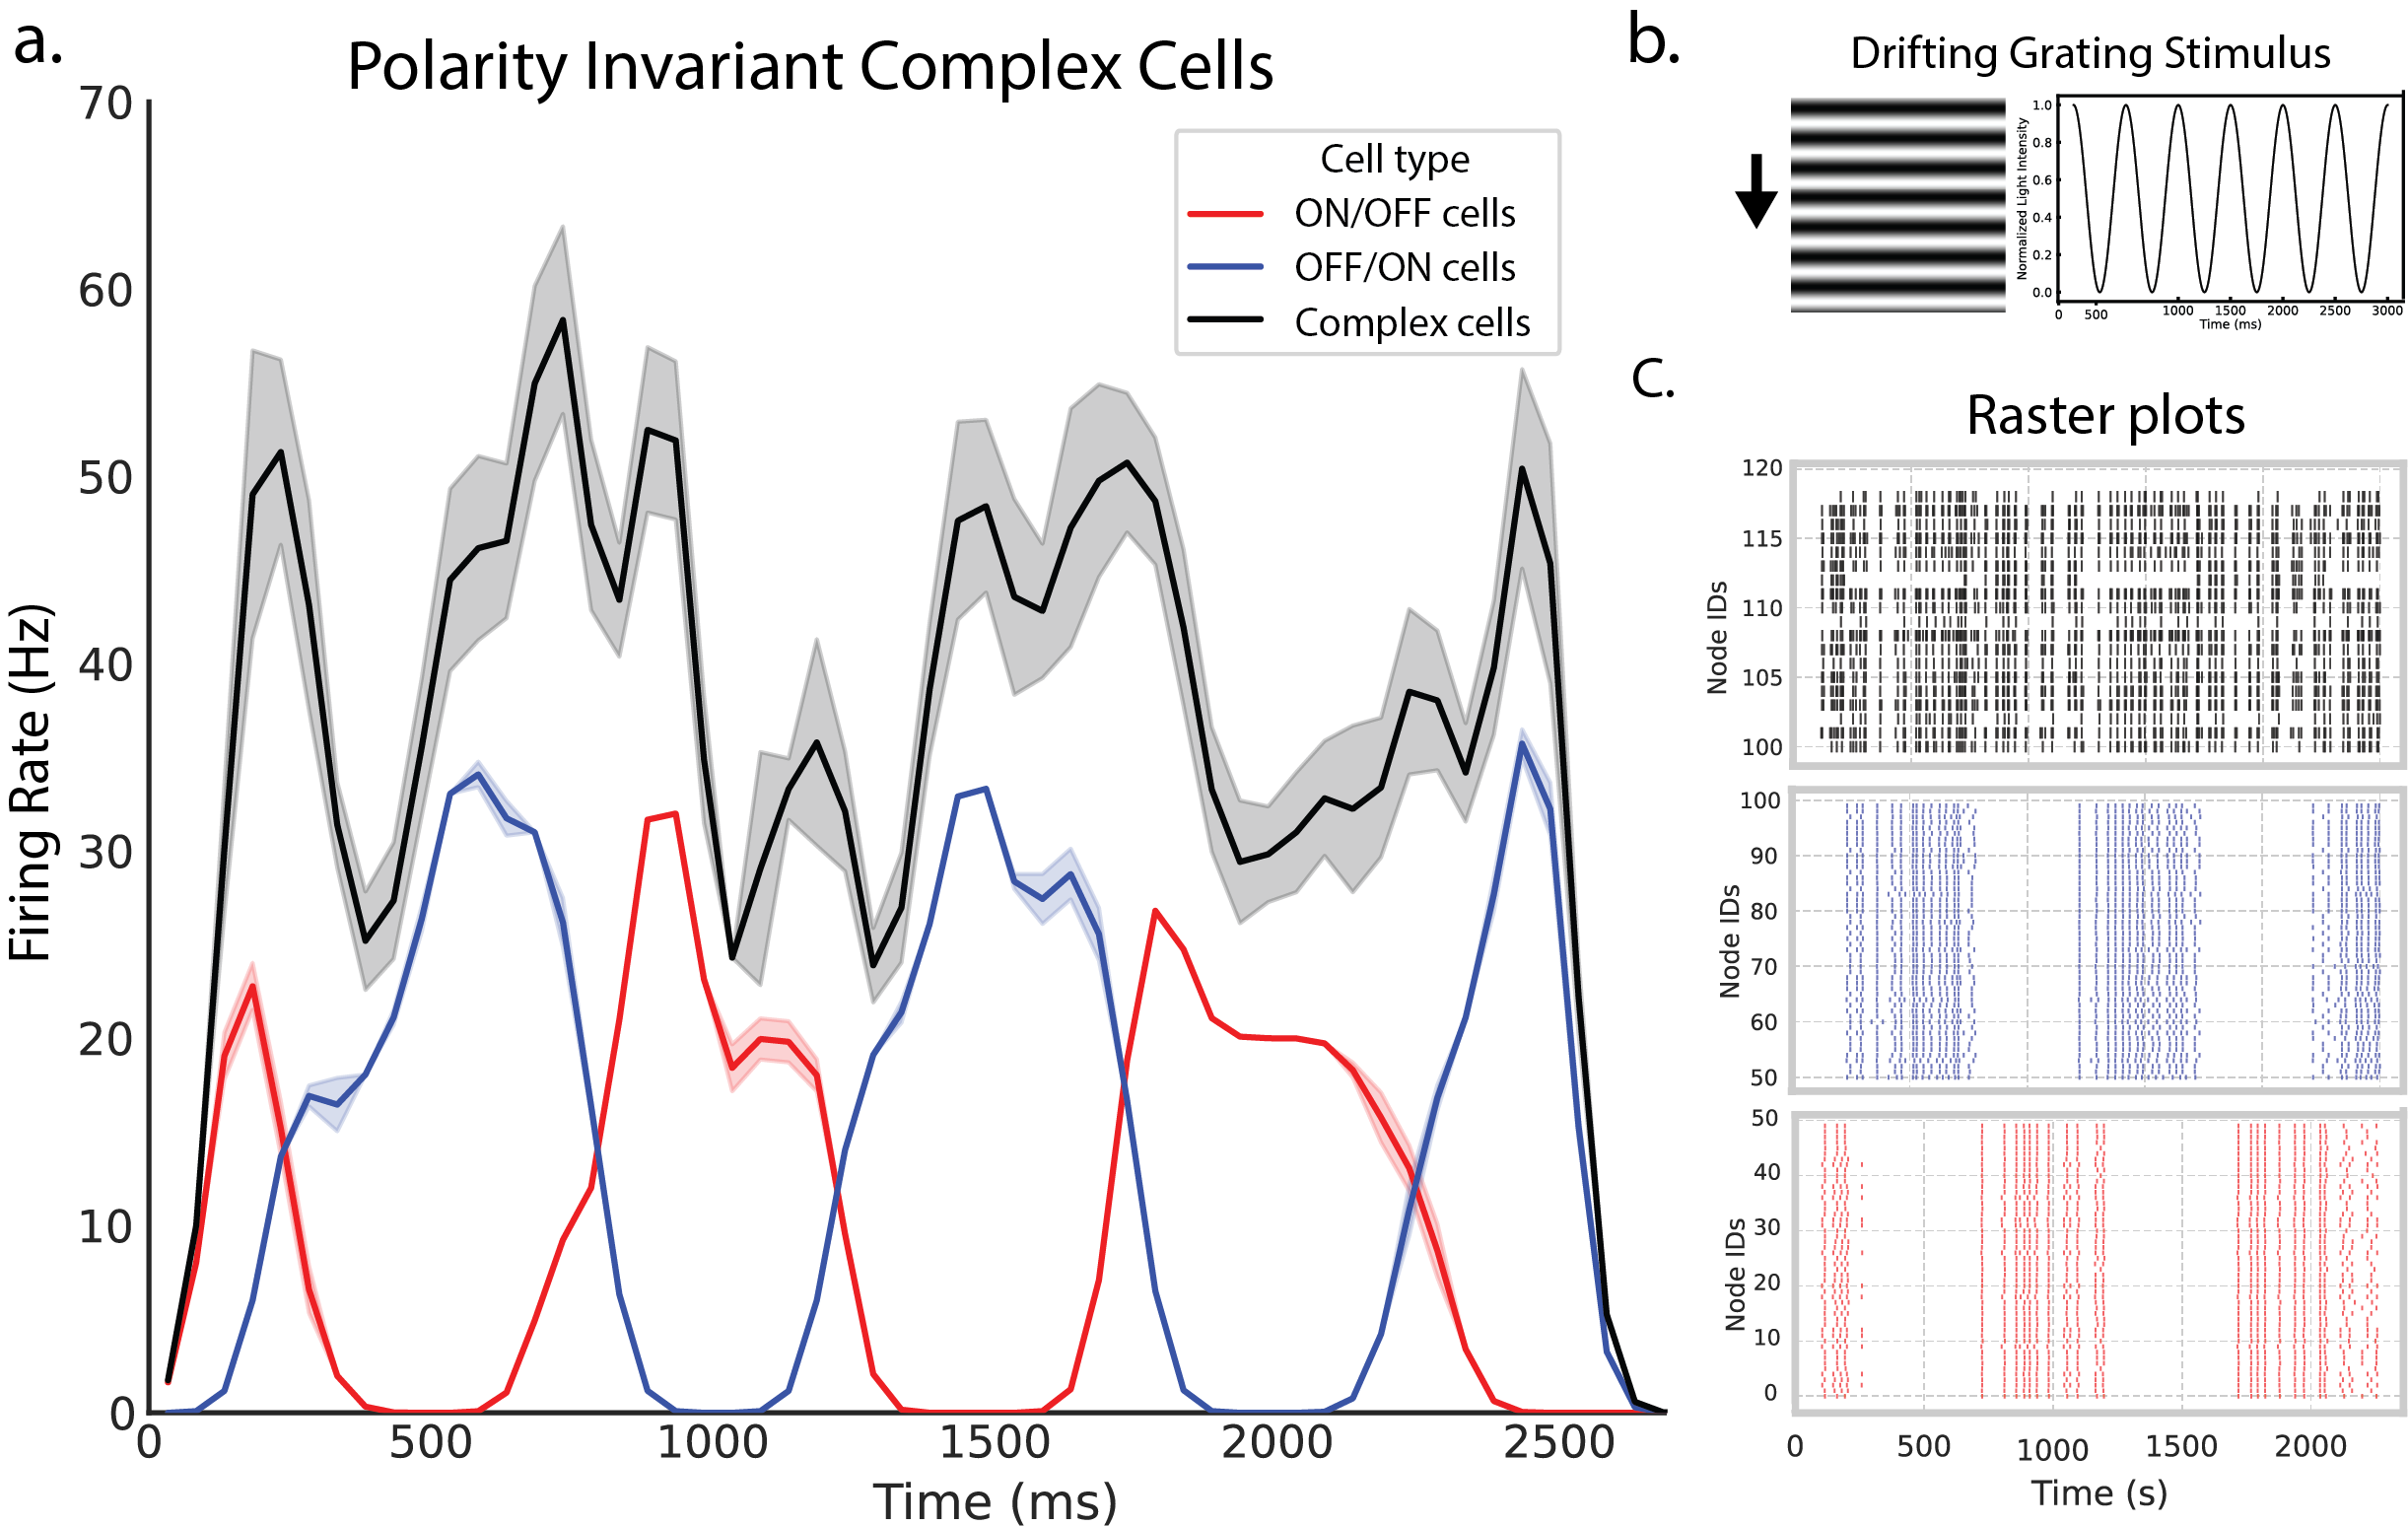
\includegraphics[width=1 \textwidth]{figures/complex_invariance_figure.png}
    \caption{a. Simple and complex cells responses to a horizontal drifting grating. ON/OFF simple cells are shown in red with an offset phase from the OFF/ON cells. The black complex cells do not exhibit the same phase sensitive. b. The drifting grating stimulus that was presented to the model. c. The raster plots also illustrate the phase sensitivity of the simple cells and how the complex cell has a stable firing to a constantly fluctuating input.}
    \label{fig:polarity invariance}
\end{figure}

%\subsection{Recurrent feedback underlying endstopping.}
Currently, only dLGN, simple cells, and complex cell were described. With these cell types one of the goals of the model was to experiment with different ways that stable endstopping could be created. In the initial phases an attempt was made to create endstopping by combining spatially offset simple cells to create endstoping in an strictly excitatory manner. The idea was to converge specific simple ON and OFF fields relative to each other, modelling the inhibitory subfield of an endstopped cell with an OFF field and the excitatory subfield with an ON field. While this method reduced the firing rate, it did not achieve a nulled spiking rate for long inputs. The main problem was that due to the excitatory nature you could only lose maximally half the input based on polarity. To remedy this and create endstopped cells that could be inhibited to complete silence, in subsequent methods, we first integrated the simple ON/OFF streams into complex cells before introducing spatial relationships between cells. And then, to create orientation-selective and phase-invariant cells that exhibit endstopping behaviour, we used recurrent activation of inhibitory cells to model this critical feature of visual processing. Thus, simple cells with orientation-selective receptive fields were connected to complex cells with similar preferred orientations that integrated inputs across different spatial phases, thus achieving phase invariance. The next step involved a laterally displaced complex cell. This neighbouring complex cell then projected to a population of inhibitory interneurons that was connected to the original simple cell population\hyperref[fig:LIF_Overview]{figure 3c}. This displacement was crucial as it introduced a spatial offset between the excitation source and the location where inhibition would be applied. The inhibitory interneurons targeted by these projections played a key role in modulating the activity of the simple cells. Once activated by the complex cells, the inhibitory cells provide feedback to the simple cells positioned in the retinotopically overlapping area of the original complex cells. This feedback loop was designed to suppress the activity of the simple cells when a stimulus extended beyond their receptive field. In more detail, as a line or bar stimulus moved across the receptive field of a simple cell and extended beyond it, the laterally displaced complex cell would activate the inhibitory interneurons. These interneurons, in turn, would inhibit the simple cells, thereby reducing their firing rate. This rapid inhibition is a hallmark of endstopping, where the neuron's response is curtailed when a stimulus exceeds the optimal length within its receptive field. The introduction of this recurrent feedback mechanism was essential for creating endstopped cells, which are specialised for detecting the endpoints of lines and bars. Endstopped cells are known for their ability to signal the presence of corners, line ends, and other salient features in the visual field, making them critical for complex shape and motion perception. By implementing this feedback loop, the model could replicate the rapid decline in firing rate that characterises endstopping, providing a more accurate and nuanced representation of visual processing as seen in the primary visual cortex. This approach highlights the importance of inhibitory feedback in fine-tuning the responses of neurons to visual stimuli, ensuring that the network could adapt to varying stimulus lengths and shapes. To investigate further how endstopped cells can be effectively integrating by higher visual areas, the same neural architecture can be used with neural populations instead of individual LIF cells. 

%ToDo change exc inh etc. to population names
\begin{table}[h]
  \centering
  \caption{Connection Weights in the LIF endstop Circuit}
  %\label{tab:weights}
  \begin{tabular}{@{}llc@{}}
      \toprule
      \textbf{From} & \textbf{To} & \textbf{Weight} \\ \midrule
      Excitatory (e) & Excitatory (e) & 0.8 \\
      Excitatory (e) & Inhibitory (i) & 2.5 \\
      Inhibitory (i) & Excitatory (e) & -3.0 \\ \bottomrule
  \end{tabular}
\end{table}

%\subsection{Population activity and illusory contour representation.}
The population models allowed us to recreate the interlaminar endstopping microcircuits by treating each cell type as a specific population and study how multiple endstopping microcircuits collectively encoded the presence of illusory contours in a specific retinotopic coordinate of the visual field. This way we still captured the dynamic interactions between simple, complex, endstopping, and inhibitory interneurons, while providing a network of which the activity could be further integrated in a higher visual cortical area such as lateromedial cortex (LM), the second visual area in the mouse. In turn, this allowed us to examine how higher level visual feedback could provide information for V1 to induce an illusory filling in mechanism between retinotopic coordinates. Thus, abstracting the LIF model into a population model allowed for a more comprehensive view of how V1 processes visual information in the case of possible occlusion and how an illusory response can be generated to particular stimulus configurations. The final endstopped cells were generated across the grid with specified offsets to ensure coverage of the visual field, and each was assigned a position based on its offset values. Simple cells were derived from the complex cells, inheriting their properties, and inhibitory cells were created to modulate the activity of the simple and complex cells. Pattern cells were generated based on specified orientations and positions to represent orthogonal illusory lines compared to the endstopped cell input they received. Connections from pattern cells to complex and endstop cells facilitated the feedback mechanisms required for simulating illusory contours \hyperref[fig:illusory_filling]{figure 7}. Particular endstopped cells are active due to the horizontal inducers ending within their excitatory receptive field, without activating the inhibitory feedback loop driven by the complex cell. In turn if enough inducers are present those signals would be integrated in the LM pattern cell, with an excitatory feedback loop as a results, filling in the illusory contour between the inducers. Therefore, the current model simulates the generation of illusory contours, based multiple recurrent feedback loops, one inhibitory local for endstopping and one excitatory between V1 and LM. 
%ToDo describe connectivity patterns used to create population model.


\begin{figure}[H]
  \centering
  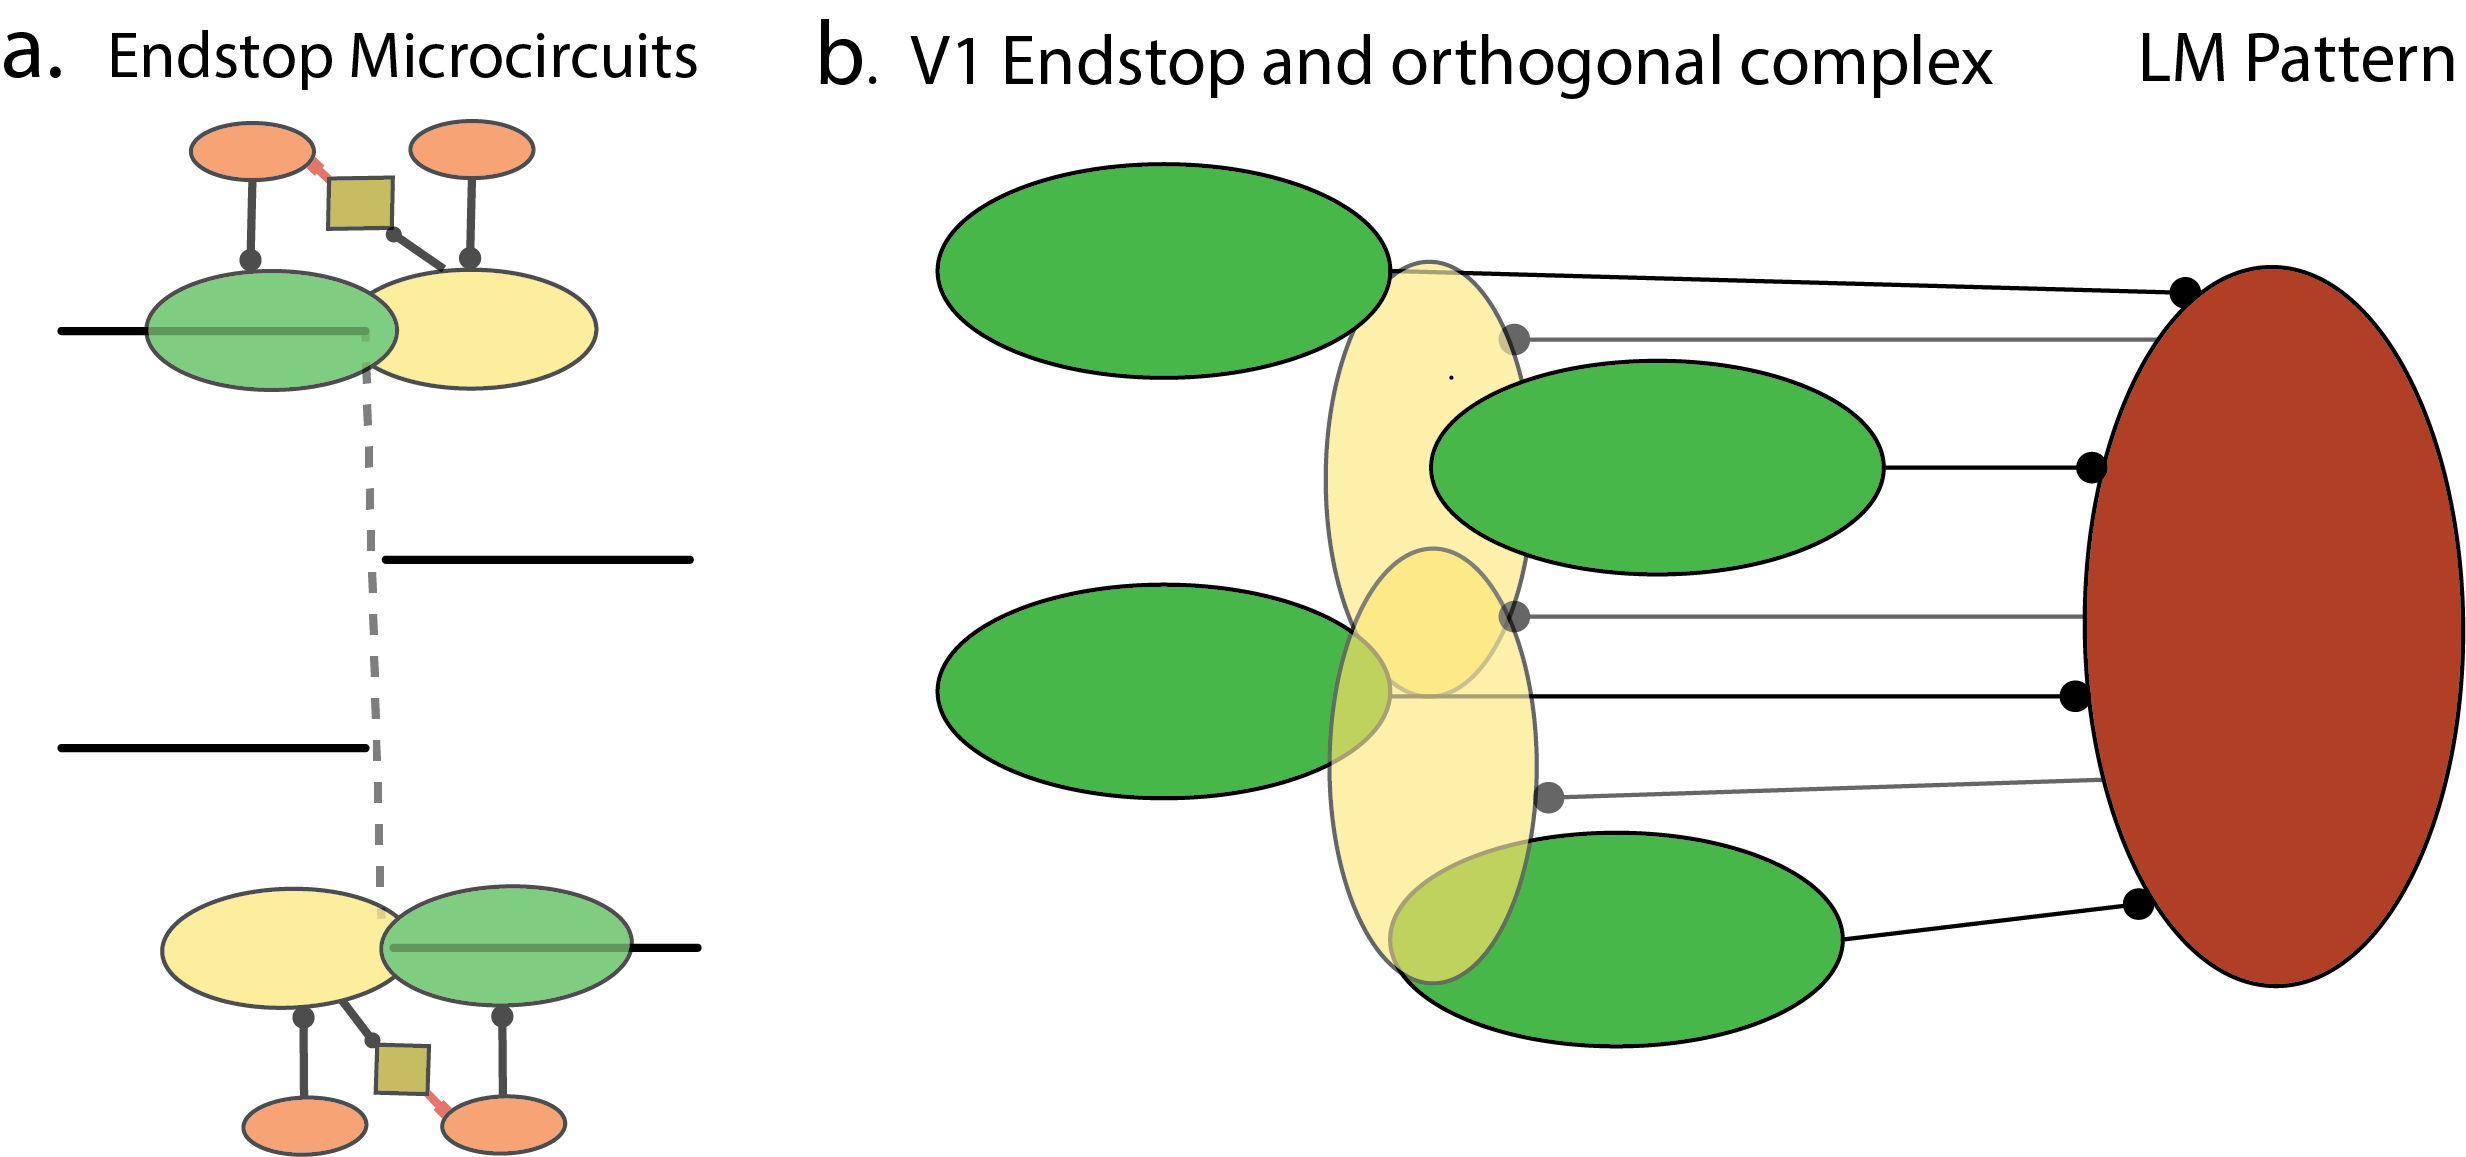
\includegraphics[width=1 \textwidth]{adjusted_figures/illusory_filling.png}
  \caption{a. The endstopped microcircuit illustrated on top of horizontal abutting grating illusion inducers. The elements that make up the microcircuit share the same retinotopic coordinates. b. If all 4 of the endstopped cells are active they fire intensely enough to activate a higher visual pattern cell in LM, which integrates these input and projects feedback onto orthogonally tuned complex cells. This way an illusory contour is locally represented through the integration of local endstopped signals.}
  \label{fig:illusory_filling}
\end{figure}

% ToDo check and rewrite
% \subsubsection{PyRates Library and population parameters.}
To use the Wilson and Cowan neural mass model within the PyRates library consists of several key components and parameters that we will explain in detail.
First, we define an operator called the synaptic excitation operator. This operator uses a sigmoid function to model the process of synaptic excitation. The equation for this operator is:
\[
m = \operatorname{sigmoid}(s \cdot (r_{\mathrm{in}} + r_{\mathrm{ext}} - \theta)) - \operatorname{sigmoid}(-s \cdot \theta),
\]
where \( m \) represents the output signal from the neuron. The term \(\operatorname{sigmoid}\) is a mathematical function that smoothly limits the output between 0 and 1, mimicking the neuron's firing rate. The parameter \( s \) controls the steepness of the sigmoid curve and is set to 1.0, meaning it defines how quickly the neuron responds to input. The parameter \(\theta\) is a threshold set to 2.0, which the input must exceed for the neuron to start firing significantly. The inputs \( r_{\mathrm{in}} \) and \( r_{\mathrm{ext}} \) represent signals coming from other neurons and external sources, respectively, and both are initially set to 0.0.
We also have a variation called the synaptic inhibition operator. This operator works similarly but models inhibitory signals, which reduce neuron activity. Its equation is similar, but with different parameters: \( s \) is set to 2.0, making the response steeper, and \( \theta \) is set to 2.5, meaning a higher threshold for inhibition.
Next, we describe the rate operator. This operator models the rate of change in neural activity over time using the differential equation:
\[
r' = \frac{-r + (1.0 - k \cdot r) \cdot m}{\tau}.
\]
Here, \( r \) is the current activity level of the neuron, initially set to 0.0. The parameter \( k \) is set to 1.0 and influences how the neuron's activity decreases over time. The term \( \tau \) represents the time constant set to 10.0, which defines how quickly the neuron activity responds to changes. The input \( m \) is the signal calculated by the excitation or inhibition operators.
To model neural populations, we use node templates. The excitatory population node template combines the rate operator and the synaptic excitation operator to represent a group of excitatory neurons, which promote activity in the network. Conversely, the inhibitory population node template combines the rate operator and the synaptic inhibition operator to represent a group of inhibitory neurons, which suppress activity in the network.

The node templates can be combine to form a circuit template defining the grand network structure of the model. The Wilson-Cowan circuit template that was used consists of two nodes types an excitatory population and an inhibitory types, that are connected similarly to the LIF model to induce functional variation between simple, complex and endstopped cells. The parameters used in the model are summarised in Table~\ref{tab:parameters}.

\begin{table}[h]
    \centering
    \caption{Parameters of the Wilson-Cowan Neural Mass Model}
    \label{tab:parameters}
    \begin{tabular}{@{}lll@{}}
        \toprule
        \textbf{Parameter} & \textbf{Description} & \textbf{Value} \\ \midrule
        \( s \) & Steepness of the sigmoid curve (excitation) & 1.0 \\
        \( \theta \) & Threshold for excitation & 2.0 \\
        \( r_{\mathrm{in}} \) & Input from other neurons & 5.0 \\
        \( r_{\mathrm{ext}} \) & External input & 0.0 \\
        \( s  \) (inhibition) & Steepness of the sigmoid curve & 2.0 \\
        \( \theta \) (inhibition) & Threshold for inhibition & 2.5 \\
        \( r \) & Current activity level & 0.0 \\
        \( k \) & Decay parameter for activity & 1.0 \\
        \( \tau \) & Time constant (ms) & 10.0 \\ \bottomrule
    \end{tabular}
\end{table}

The connections between these nodes are specified with weights that determine the strength and type of influence they exert on each other. The weights for these connections are as follows: the rate output \( r \) of the excitatory node feeds back into its own synaptic excitation input \( r_{\mathrm{in}} \) with a weight of 15.0, the rate output \( r \) of the excitatory node feeds into the synaptic inhibition input \( r_{\mathrm{in}} \) of the inhibitory node with a weight of 15.0, the rate output \( r \) of the inhibitory node reduces activity in the excitatory node by feeding into its synaptic excitation input \( r_{\mathrm{in}} \) with a weight of -15.0, and the rate output \( r \) of the inhibitory node also self-regulates by feeding back into its own synaptic inhibition input \( r_{\mathrm{in}} \) with a weight of -4.0. These parameters allowed us to simulate neural interactions between both excitatory and inhibitory populations. By adjusting the weights and incorporating these parameters, we can flexibly and realistically represent neural behaviour and understand how neurons interact and influence each other over time. Additionally, the connections between these nodes are specified with weights that determine the strength and type of influence they exert on each other. These weights are outlined in Table~\ref{tab:weights}. These detailed specifications allow us to simulate complex neural dynamics, capturing both excitatory and inhibitory interactions within the network. By adjusting the weights, we can flexibly and realistically represent neural behaviour and understand how neurons interact and influence each other over time.

\begin{table}[h]
    \centering
    \caption{Connection Weights in the Wilson-Cowan Circuit}
    \label{tab:weights}
    \begin{tabular}{@{}llc@{}}
        \toprule
        \textbf{From} & \textbf{To} & \textbf{Weight} \\ \midrule
        Excitatory (e) & Excitatory (e) & 7.0 \\
        Excitatory (e) & Inhibitory (i) & 7.0 \\
        Inhibitory (i) & Excitatory (e) & -14.0 \\
        Inhibitory (i) & Inhibitory (i) & -4.0 \\ \bottomrule
    \end{tabular}
\end{table}


\section*{Results}
%\subsection{LIF Endstopped Receptive Field properties.}
\setlength{\parindent}{24pt}
To investigate the role of recurrent inhibition in the process of endstopping, we developed a LIF point neuron model comprising a microcircuit of simple, complex, and inhibitory interneurons. The simple cell population at a specified retinotopic coordinate connects to a complex cell, creating an inhibitory feedback loop that suppresses the activity of a neighbouring simple cell population. This configuration allows us to simulate the behaviour of endstopped cells in response to line segments of varying lengths and orientations. The results, as illustrated in figure \ref{fig:endstopping}, demonstrate that the endstopped cell spikes maximally when a line bar is positioned over the classical receptive field. However, this activity is inhibited when the line extends into the receptive field of an adjacent complex cell, attributed to the inhibition from the recurrent inhibitory population.
\setlength{\parindent}{0pt}
\\
\hyperref[fig:endstopping]{Figure 8} demonstrated the dynamics of endstopping responses within this microcircuit model. The four subplots (a, b, c, d) represent the average firing rates of neurons exposed to bars of varying lengths (10, 15, 25, and 35 visual degrees) at four different orientations: 0°, 15°, 30°, and 45°. At 0° orientation, the firing rates exhibit a distinct pattern. The short bar of 20 visual degrees elicits the highest response, with firing rates peaking around 70 Hz between 100 and 200 ms after stimulus presentation and showing a significant sustained response beyond 1000 ms of the simulation. As the bar length increases, the firing rates decrease, indicating a strong endstopping effect. Bars of 15, 25, and 35 visual degrees show progressively lower peak firing rates and shorter durations of sustained activity, with the 35-degree bar almost not eliciting any response. Moreover, as the orientation of the presented bar increases, we observed a gradual decline in the initial firing rate as well as a balanced endstopping effect due to varying amounts of coverage of the complex receptive field when the bar is rotated. At a 15° orientation, the response pattern shifts slightly. The 15 visual degree bar still evokes the highest firing rate, but the peak is slightly lower than at 0°, around 50 Hz. The response sustains similarly; however, the relative difference between the response elicited between the 10 and 15 degrees is smaller compared to the horizontally oriented bar at 0°. This trend continues as the bar is further rotated. In figure d, the extended bar does not reach the receptive field of the complex cell, resulting in the absence of endstopping features. The endstopped cell also shows reduced sensitivity, illustrated by the peak firing rate of 20 Hz.
\\
In conclusion, the figures illustrate how bar length and orientation shape the response of endstopping neurons. The current circuit configuration supports sustained activity and has strong recurrent connections that induce endstopping even with full excitatory receptive field activation. The endstopped cell maintains orientation selectivity as length and orientation vary, showing the greatest spiking difference between bar lengths of 15 and 35 degrees and rotations of 0 and 45 degrees. Additionally, the results indicate that as angles steepen, length sensitivity gradually decreases while orientation effects become more pronounced, resulting in lower peak firing rates and thereby a relative decrease in endstopping behaviour.
% In conclusion, the figures illustrate the interaction between bar length and orientation in shaping the response of endstopping neurons. The findings emphasise that the current circuit configuration can sustain activity as an averaged population and have recurrent connections strong enough to induce endstopping even when the excitatory receptive field is entirely activated. The orientation selectivity of the endstopped cell remains intact when length and orientation vary, with the preferred orientation inducing the most significant relative spiking difference between bar lengths of 15 and 35 degrees and between 0 and 45° rotation. Furthermore, the results show that at steeper angles, length sensitivity decreases gradually, and orientation effects become more pronounced, with decreasing peak firing rates as a result.
% ToDo: add phsyiological recording of endstopping and put next to it, cat receptiv fields smaller than mouse. so discuss why it is different
\vspace*{-\headsep}
\vspace*{-\headheight}
\vspace*{-60pt} % Adjust the value to move the figure up
\begin{figure}[H]
    \centering
    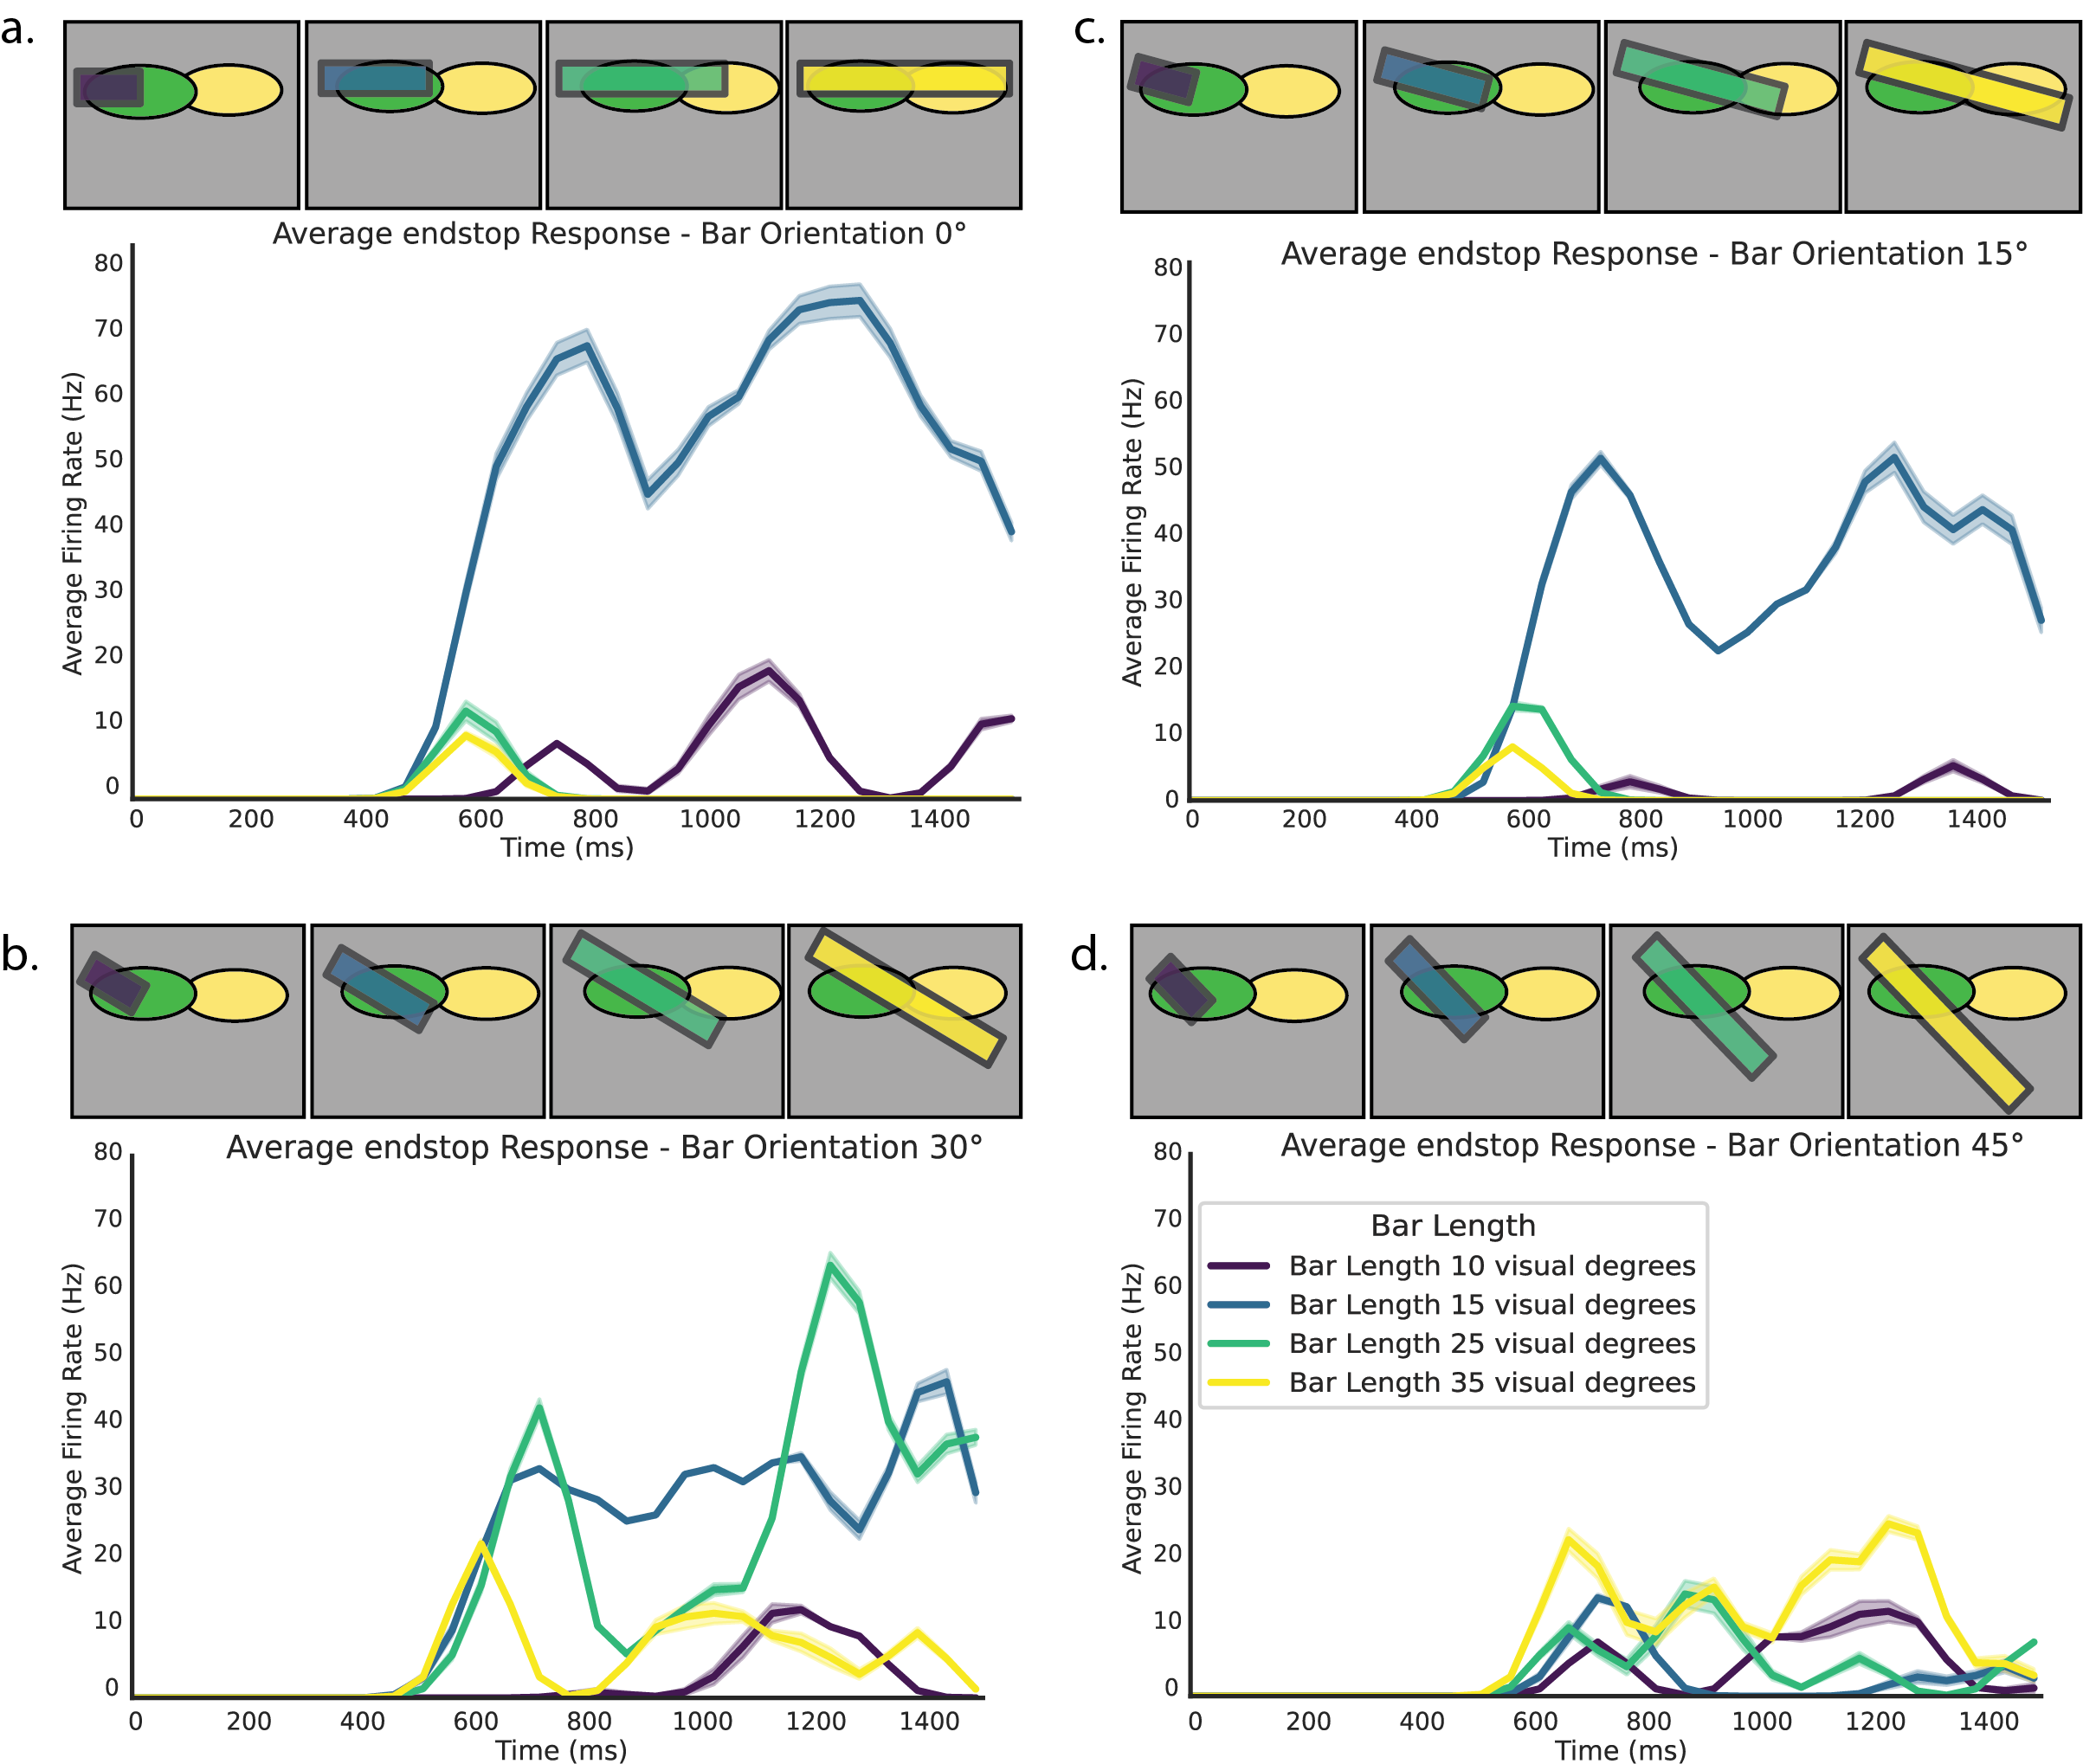
\includegraphics[width=1.0 \textwidth]{./figures/LIF_endstopping_length_orientation.png}
    \caption{Responses of the endstopped complex cells to different line segment lengths. The x-axis represents the length of the line segment in visual degrees, and the y-axis represents the firing rate of the complex cell in spikes per second (Hz). The cell types are colour coded of which the legend is located in d. The endstopped cell has an orientation preference of 0 degrees rotation, which is presented in figure a. The relative difference between bar lengths is greatest in this figure. Other figures show that with a greater orientation, peak firing rates decrease and that relative firing rate difference between bar lengths also decreases with more rotation. In panel e. and f. the response of a real hypercomplex cell in cat visual cortex for different orientation is plotted. The receptive field of endstopped cells is smaller compared to those found in mice.}
    \label{fig:endstopping}
\end{figure}

To gain a better understanding of the neural dynamics within the circuit, we also stimulated the model with a continuously growing bar. This approach allows us to visualise subtle differences related to the length of the bar at the population's preferred orientation, as shown in \hyperref[fig:endstopping_length]{figure 9a}. This figure illustrates the elicited response of endstopped neurons to a bar that starts at the beginning of the receptive field and extends progressively into the endstopping inhibitory endzone. The lineplot on the left shows the average firing rate in spikes per second (Hz) of the endstopped neurons as a function of bar length in visual degrees. The shaded area represents the variability around the mean firing rate. As depicted, the average firing rate increases steadily as the bar lengthens from 0 to approximately 15 visual degrees, peaking around 70 Hz. This peak indicates the optimal bar length that maximally activates the endstopped neurons within the receptive field. Beyond this length, the firing rate starts to decline, reflecting the inhibitory effect as the bar extends into the adjacent complex cell's receptive field.
\bigbreak
The insets on the right side of the figure provide a visual representation of the bar's interaction with the receptive fields at different stages of its growth. The top inset shows the bar initially positioned within the receptive field of the endstopped neuron, eliciting a strong response. The middle inset illustrates the bar extending into the inhibitory zone, where the inhibitory feedback begins to reduce the firing rate. Finally, the bottom inset depicts the bar fully extending into the adjacent complex cell's receptive field, resulting in a significant reduction in the firing rate due to maximal inhibition. This figure effectively captures the dynamic response of endstopped neurons to varying bar lengths, highlighting the intricate balance between excitation and inhibition within the microcircuit. It reinforces the notion that recurrent inhibition plays a crucial role in modulating the activity of endstopped neurons, particularly in response to stimuli that extend beyond their classical receptive fields.

  \begin{figure}[H]
    \centering
    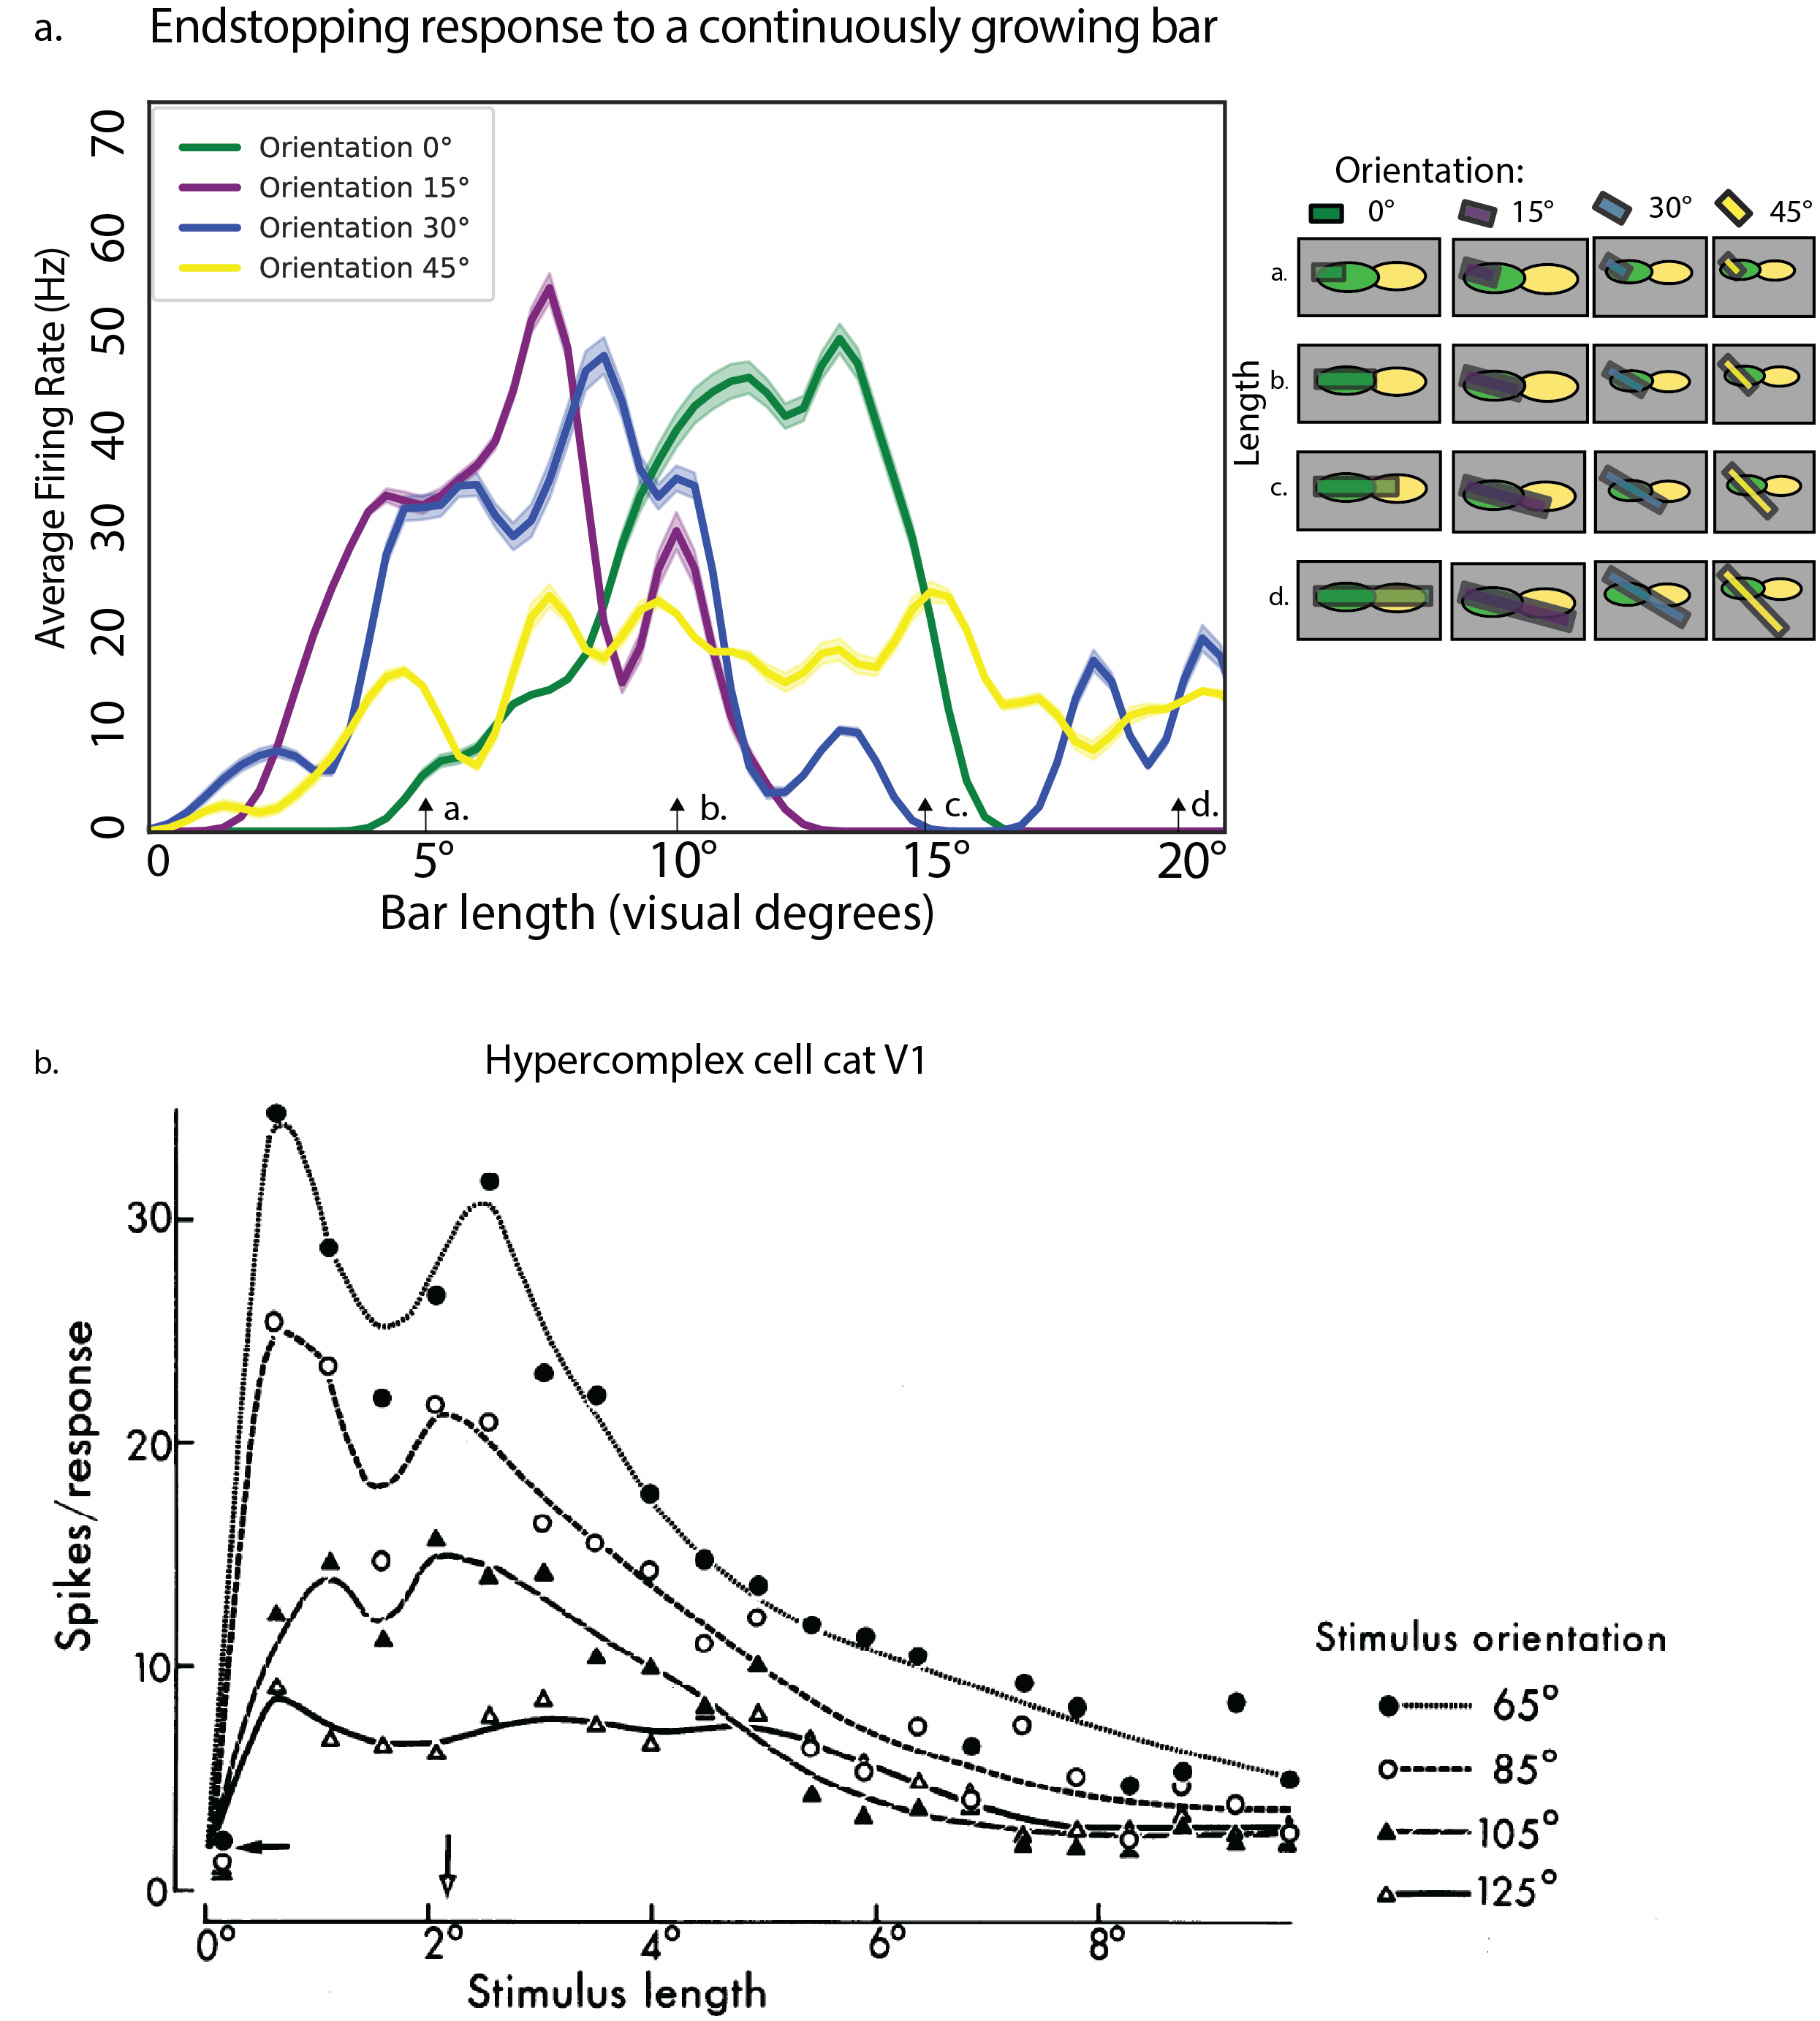
\includegraphics[width=1.0 \textwidth]{adjusted_figures/endstop_line_length_physiology.png}
    \caption{The response of an endstopping population stimulated with a continuously growing bar. Firing rates increase until the stimulus bar exceeds 15 visual degrees, after which firing is quickly dampened for longer inputs.}
    \label{fig:endstopping_length}
  \end{figure}

  %ToDo rewrite population model description
%\subsection{Population activity illusory contours}
Next, we examined whether our population model reflected results found during physiological experiments done with the abutting grating illusion \autocite{vonderheydtMechanismsContourPerception1989}. They showed that the illusory contour breaks down when a gap is introduced misaligning the horizontal inducers. Additionally, they demonstrated that when a bar crosses the illusory line illusory responses decreased as well. Figure \ref{fig:population_contours} showcases the responses of different cell types to visual stimuli designed to induce the perception of illusory contours. The left panels of each sub-figure (a, b, and c) display the mean firing rates of various cell populations, including complex cells tuned to 90 degrees for the illusory response, complex cells tuned to 0 degrees that are tuned for the inducers and to create endstopped cells, and pattern cells used to integrate signals from the endstopped cells. The right panels depict the spatial arrangement and the type of stimulus presented, which varies across the sub-figures.
\bigbreak
% In subfigure (a), the stimulus arrangement created a strong illusion of contours aligned with the orientation preference of the complex 90 cells. This is evidenced by the robust mean firing rate of the complex cells tuned to 90 degree orientations peaking at around 30 Hz, indicating a high level of activity in response to the perceived illusory contours. The elevated firing rates suggest that these cells are effectively encoding the illusion, signaling the presence of a boundary where none exists in the physical stimulus. When the stimulus is altered to disrupt the illusion, as seen in subfigures (b) and (c), the activity of the complex 90 cells changes significantly. In subfigure (b), the stimulus modification appears to partially disrupt the illusory contour. This is reflected in the reduced firing rate of the complex cells tuned to 0 degree input compared to subfigure (a), though the response remains notable. This partial disruption suggests that the illusory contour is weakened but not entirely broken, resulting in a moderate decrease in the encoding efficiency of these cells.

In subfigure (a), the stimulus created a strong illusion because inducers were horizontally in the orientation preference of complex 0° cells and were vertically aligned, so the pattern cell was maximally stimulated. The robust mean firing rate of the complex 90° cells, peaking around 40 Hz, suggested effective encoding of the perceived illusory contours. When the stimulus is modified in sub-figures (b) and (c) to disrupt the illusion, the complex 90° cells' activity changes significantly. Sub-figure (b) shows a partial disruption of the illusion, reflected in a reduced firing rate of the complex cells, though the response remained around baseline, indicating a potential for illusory contour but not enough to effectively activate the pattern cell population.
\bigbreak
In sub-figure (c), the stimulus is further modified, to completely break the illusion. The firing rate of the complex 90° cells drops significantly compared to sub-figures (a) and (b). This substantial reduction in activity indicates that the complex 90 cells are no longer effectively encoding the illusory contour, as the stimulus no longer supports the perception of such a contour. The response of these cells now aligns more closely with their response to an actual absence of contours, highlighting their role in specifically detecting and encoding illusory boundaries. The right panels of each sub-figure visually illustrated the stimulus configurations, showing how the spatial arrangement of elements impacts the perception of illusory contours. The colour coding indicates the average firing rates, with warmer colours representing higher activity levels. The complex cells (dotted outlines) and end-stop cells (solid outlines) are shown in their spatial positions, providing a visual representation between cell type, location, and stimulus-induced activity.
\bigbreak
In summary, the complex 90 cells are crucial for encoding illusory contours, as evidenced by their high firing rates in response to stimuli that induce such perceptions. When the stimulus is altered to disrupt the illusion, the activity of these cells decreases accordingly. This suggests that the complex 90 cells are finely tuned to detect and encode the presence of contours, whether real or illusory, and their activity is a direct reflection of the strength of the perceived illusion. These findings underscore the importance of specific neural populations in the higher-order processing of visual information, particularly in the context of perceptual phenomena like illusory contours.

\begin{figure}[H]
  \centering
  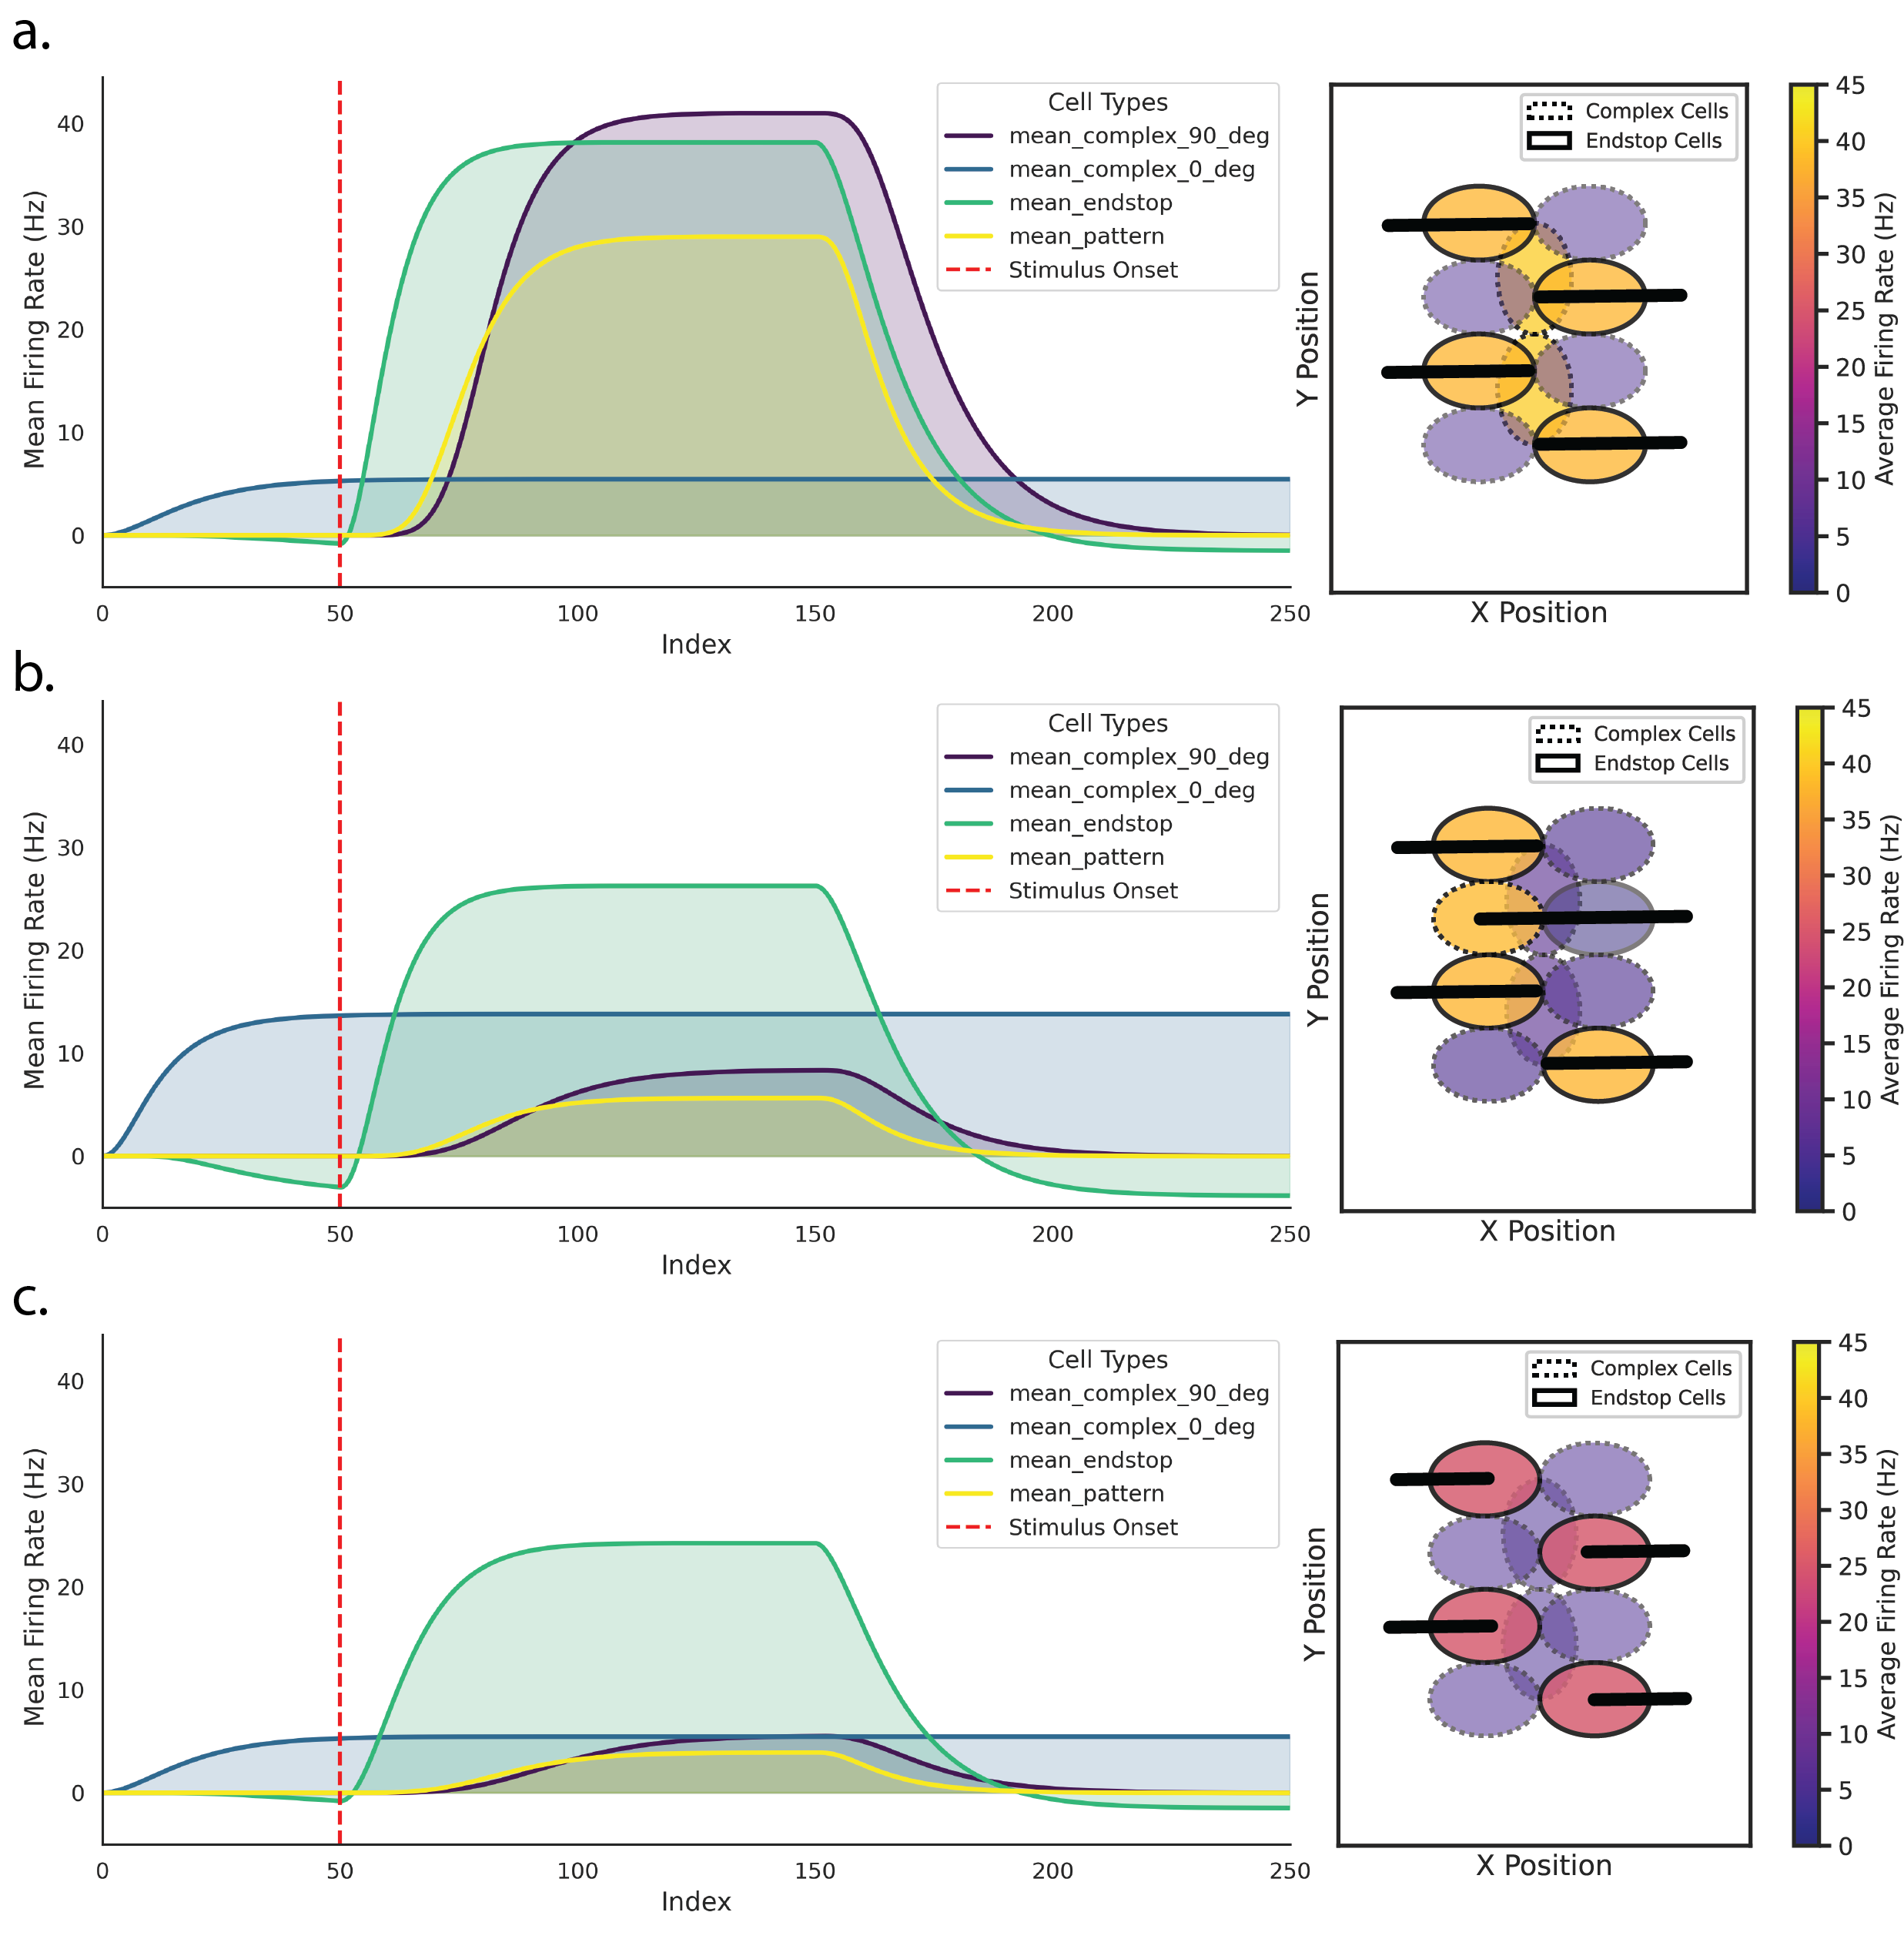
\includegraphics[width=1.0 \textwidth]{figures/Figure_Population_configs.png}
  \caption{a. The optimal input is given to the model, all inducers are the preferred orientation and are spatially aligned. All endstopped populations are very active and the complex endzones are not active, thus resulting in maximum representation of the illusory contour. b. In this example one of the inducers crosses the illusory contour, resulting in the abolishment of the illusion. The complex endzones increase in activity and thus is the endstopped cell decreased and no illusory contour is formed. c. Similarly, in this figure the inducer lines are not aligned enough the form a strong illusory contour. The complex endzones are not activated, but also the endstopped cells are not maximally stimulated. Therefore, the pattern cell is not stimulated enough and no illusory contour is formed.}
  \label{fig:population_contours}
\end{figure}

% %\subsection{Representation real contours vs illusory contours in the model}


\newpage
\section*{Discussion}
\setlength{\parindent}{12pt}  
The current models demonstrated that endstopping can be generated through recurrent inhibitory connectivity and can be effectively integrated by higher visual areas to drive recurrent contour completion. We modelled endstopped cells by creating a LIF microcircuit of two adjacent populations of complex cells connected through inhibitory feedback on the simple cell level. The inhibitory feedback resulting in a decrease in firing whenever a stimulus edge is extended beyond the excitatory endstop receptive field into the inhibitory endzone. This LIF model demonstrated that the endstopped cells are a critical first step for the detections of illusory inducing local features. To examine how the global representation of the aubtting grating illusion is formed we used a second model that implemented population mass firing rate model equations. This population model had a similar architecture that was used in the LIF model, but with the extension of a higher visual area LM. The abstraction from point neurons to neural populations ensured a stable firing rate without the need for extensive weight tuning between individual cells. Still, the population model had a similar architecture as compared to the LIF model; in which endstopping microcircuits were made from combined simple, complex, and inhibitory cells. Results from the population model demonstrated that endstopped signals can be used to group retinotopically aligned inducers into a global illusory representation by recurrently amplifying feedback signals originating from LM. 
\setlength{\parindent}{0pt}
\bigbreak


%no direct inhibition (check the original paper: silito 1977), why not? recurrent inhibition plays a role in balancing activation  \autocite{znamenskiyFunctionalSpecificityRecurrent2024}, \autocite{hanselMechanismOrientationSelectivity2012}
% Results from the LIF model showed that recurrent inhibitory signals can be used to generate endstopping behaviour robust to stimuli variations of length and orientation. Functional connectivity studies in mouse V1 have found that inhibition can stabalise excitatory activity ()
% See how Skotton shows that orientation selectivity chagnes endstopping (Skottun 2005, \autocite{orbanDimensionsPropertiesEndzone1979})
%\subsection{Recurrent inhibition stabilises endstopping.} 
%1- endstopped cells are excitatory and inhibitory endzones are indirect
% 2- Results demonstrate gradual decline in endstopping while varying input features, physiologically relevant see Orban dimension properties 1979.
% 3- No direct inhibition Silitio 1977, maybe indirect inhibitory recurrency can have stabilising effects Znamenskiy 2024 and hansel 2012 
%4- the indirect inhibition of complex endstopped cells might explain the second order spiking features yazdanbakhs 2006.
% 1.
% Inhibition plays a vital role in both the LIF and population models, PV interneurons play a major role in visual processing, shaping how sensory information is processed. In the context of the LIF model, endstoped cells are influenced by direct excitation from feedforward inputs and indirect inhibition through recurrent feedback connections. These inputs form distinct receptive fields, a feedforward classical receptive field and a retinotopically offset receptive field that functions as an inhibitory endzone. In alignment with observations from \textcite{sillitoContributionExcitatoryInhibitory1977}, inhibitory influences are not exerted directly at the level of the endstopped cells. We propose that the segregation of inhibition serves a functional purpose to generate stable endstopping. Current results showed by varying the stimulus length and orientation that endstopping is gradually reduced when stimuli diverged from its optimal configuration, and we propose that PV interneuons play a pivotal role in moderating excitatory and inhibitory interactions. The indirect inhibitory feedback, facilitated by PV interneurons, allows for a more adaptable and nuanced modulation of the excitatory signals depending on the visual context. This adaptive modulation is crucial, especially when the visual stimuli vary in length and orientation, leading to changes in the perceived endstopping effect. The dynamic regulation by PV interneurons helps maintain a balance that can prevent excessive excitatory activity that might otherwise lead to neural saturation or noise dominance in the signal processing.

% Moreover, the organisation of synaptic weights in PV interneurons as described by \textcite{znamenskiyFunctionalSpecificityRecurrent2024}, highlights the functional benefits of indirect inhibition used in the current model. By preferentially inhibiting those pyramidal neurons that share similar visual selectivities and provide strong excitatory feedback, PV interneurons not only suppress potential excitatory overshoots but also enhance the overall selectivity and sharpness of neural responses. This targeted inhibition is essential for refining the output of neural assemblies, ensuring that the response patterns are both specific and contextually appropriate. Furthermore, indirect inhibitory effects might be able to explain why endstopped cells exhibit contrast sensitivity in their second order spiking features.

Inhibition plays a vital role in both the LIF and population models, where PV interneurons play a major role in visual processing, shaping how sensory information is processed. In the context of the LIF model, endstopped cells are influenced by direct excitation from feedforward inputs and indirect inhibition through recurrent feedback connections. These inputs form distinct receptive fields, a feedforward classical receptive field and a retinotopically offset receptive field that functions as an inhibitory endzone. In alignment with observations from \textcite{sillitoContributionExcitatoryInhibitory1977}, inhibitory influences are not exerted directly at the level of the endstopped cells. We propose that the segregation of inhibition serves a functional purpose to generate stable endstopping. Current results showed by varying the stimulus length and orientation that endstopping is gradually reduced when stimuli diverged from its optimal configuration, and we propose that PV interneurons play a pivotal role in moderating excitatory and inhibitory interactions. The indirect inhibitory feedback, facilitated by PV interneurons, allows for a more adaptable and nuanced modulation of the excitatory signals depending on the visual context. This adaptive modulation is crucial, especially when the visual stimuli vary in length and orientation, leading to changes in the perceived endstopping effect. The dynamic regulation by PV interneurons helps maintain a balance that can prevent excessive excitatory activity that might otherwise lead to neural saturation or noise dominance in the signal processing.

Moreover, the organisation of synaptic weights in PV interneurons, as described by \textcite{znamenskiyFunctionalSpecificityRecurrent2024}, highlights the functional benefits of indirect inhibition used in the current model. By preferentially inhibiting those pyramidal neurons that share similar visual selectivities and provide strong excitatory feedback, PV interneurons not only suppress potential excitatory overshoots but also enhance the overall selectivity and sharpness of neural responses. This targeted inhibition is essential for refining the output of neural assemblies, ensuring that the response patterns are both specific and contextually appropriate. Furthermore, the ability of endstopped cells to adjust their firing patterns based on contrast variations could offer insights into the mechanisms underpinning contrast sensitivity in their second order spiking features, suggesting a complex interplay between inhibition and sensory perception.

%Talking about the comparison to physiology endstopped cells of the cat


%\subsection{Recurrent inhibition can provide endstopped cells with information about sign of contrast.} % simple cell \autocite{yazdanbakhshEndStoppingV12006}
Endstopping is observed in both simple and complex cells within the visual cortex, presenting a paradox within complex cells where it is traditionally assumed that information about the sign of contrast has already been pooled making this information inaccesible for later stages \autocite{yazdanbakhshEndStoppingV12006}. This presents a challenge since endstopping at the complex cell level, crucial for visual interpretation. Despite this presumed pooling, complex cells exhibit sensitivity to the sign of contrast, distinguishing between reversed contrast conditions at stimulus junctions \autocite{yazdanbakhshEndStoppingV12006}. This capability is vital for accurately identifying the end of a contour, essential for processing scenes with complex visual elements like shadows, transparency, occlusion, and neon colour spreading, where contrast distincly change at junctions. A possible resolution of this paradox may lie in the role of recurrent inhibition, which in our model modulates the responses of complex cells and allows for endstopping. If endstopped cells are capable of transmitting information about sign of contrast that would enhance the visual system's ability for surface stratification and border ownership, ultimately interpreting visual scenes correctly without explicit junction detectors. In the current model the inhibitory endzones of the endstopped cells are governed by complex cells, however functional studies have also found simple cells that exhibit length tuning \autocite{andersonMembranePotentialConductance2001}. Within the structure of mouse V1 where simple and complex cells are found in all layers, endstopped cells can also get recurrent inhibitory signals from simple cells instead of only complex. If this is the case the recurrent inhibition would be tuned to a particular contrast and would give the endstopped cell the information needed to interpret sign of contrast. This would allow the visual system's to easier segment an image in three-dimensions enhancing neuronal grouping and determining border ownership. More research is needed to determine the exact inputs that an endstopped cell receives. Also, to further examine how the convergence of endstopped cells can facilitate illusory contours it is necessary to examine the processing and feedback projections from higher visual areas.


%\subsection{Excitatory recurrent connections drive feature specific boundary completion}
  % (Population) LM pattern cell grouping local features to build robust representation, driven by recurrent excitation of endstopped cells.}
In addition to local inhibitory recurrent connections in V1, there are also excitatory recurrent connections found between area LM and V1 \autocite{muirSpecificExcitatoryConnectivity2017}. The research conducted by \textcite{muirSpecificExcitatoryConnectivity2017} provides compelling insights into the excitatory recurrent pathways between LM and V1, illustrating how these excitatory recurrent connections are not merely simplistic like-to-like mappings but rather engage in feature-binding responses to plaid stimuli, suggesting that a network of local recurrent circuitry allows for dynamically shaping perceptual outputs based on composite visual inputs. Additionally, in work by \textcite{marquesFunctionalOrganizationCortical2018}, they observed that feedback connections from LM to V1 preferentially targeted retinotopically matching location, however that orientation selective axons spread around the location perpendicularly to their preferred orientation. These findings are in line with predictions from the current model that highlights how direct feedback from LM to V1 could induce a perpendicular illusory contour if there is sufficient local recurrent activity. Complementing this, the study by \textcite{shinRecurrentPatternCompletion2023} extends our understanding by demonstrating the functional significance of these recurrent pathways in the processing of illusory contours within V1. Their experimental evidence shows that V1 neurons are integral not only in responding to direct sensory inputs but also in actively reconstructing visual information through recurrent interactions. These neurons enhance the perception of illusory contours, effectively recreating V1 activity in the absence of explicit external cues, thereby highlighting the essential role of recurrent connectivity in supporting sensory illusions and perceptual consistency of occluded figures. Feedback would in this case be orientation specific, however it might be physiologically beneficial for feedback projections to be broadly tuned.
% % Ji, Gamanut, Burkhalter, 2015. Modularity in the organisation of mouse V1; no clustering retinotopic equivalence but integrating distant
% Additionally, the population mass neuron model predicts that complex cells, rather than  inhibitory V1 cells are the primary target of feedback signals that are responsible for the resulting illusory boundary completion. Additionally, population models demonstrated accurate responses to stimulus configurations that are close to eliciting an illusory response, however are varied, so they should not. Altogether, these findings indicate that recurrent activity induced by endstopping cells is essential for the robust segmentation of the abutting grating illusion. Additionally, population models showed that endstopped signals are sufficient to guide population activity to fill in details that are not present in the local feedforward input, but have behavioural relevance due to the collective meaning of the stimulus configuration, such as the representation of a visually occluded object.

%\subsection{Broadly tuned feedback allows for the representation of curved illusory contours}
The current architecture of our population model utilises feedback connections that exhibit a highly selective, like-to-like connectivity pattern. Although this scheme is effective for basic feature detection, it potentially limits the model's capacity to integrate complex visual stimuli into coherent perceived objects. Inspired by the computational findings of \textcite{muirSpecificExcitatoryConnectivity2017}, we propose an expansion of this framework that incorporates a more dynamic feedback mechanism that integrates more broadly. Their seminal work illustrated how specific orientations could converge through recurrent connections and hierarchical processing to integrate different orientation bars into a unified plaid pattern. Emphasising the potential for sophisticated integration strategies beyond simple feature alignment. Expanding upon this, our proposed model modification involves broadening the feedback projections to encompass a wider range of orientations within a specific retinotopic area. By doing so, recurrent excitation could be leveraged to amplify the interactions between overlapping orientations, thereby enriching the model's ability to generate and interpolate complex visual structures. This feedback mechanism would allow for the formation of curved surfaces and the interpolation between non-orthogonal points—capabilities that are currently absent in our model but are crucial for mimicking a more realistic and robust visual perception process. This approach not only aligns with the physiological evidence suggesting that the visual cortex utilises broad, integrative feedback mechanisms to refine perceptual outputs but also opens new avenues for modeling how the brain interprets and reconstructs complex visual scenes from sparse inputs. By enabling the model to interpolate illusory contours more effectively, we anticipate a significant improvement in its ability to reconstruct detailed and continuous visual experiences from fragmented or partially occluded stimuli. 

%\subsection{Improving network stability with deep learning optimisation strategies}
  % Deep learning strategies can help present many input, have the receptive fields be created through deep learning. To test hypothesis define the feedforward input architecture and find out what feedback structure the model comes up with when creating illusory contours.}
One limitation in the current work is that most of the tuning was done by hand. This makes it increasingly hard to tune recurrent connections and intricate feedback mechanisms. To prevent this in future research deep learning strategies have to be utilised in order to tune weights by presenting large datasets of input to the model. By harnessing the power of neural networks, researchers can explore how visual systems interpret incomplete information to form coherent percepts and allow the data to learn from the data. This will allow for creative solutions that would be impossible to create by hand. At the heart of the current models lies the concept of recurrent endstopping, this feedforward model can be specified for the algorithms to be lead into a particular direction. Thereby providing a foundational framework for constructing deep learning models that simulate this complex perceptual task in a way that is biologically plausible.
\\
In a typical deep learning framework designed to capture the essence of illusory contour detection, a convolutional neural network (CNN) can be employed due to its efficacy in handling image data and its architectural mimicry of the hierarchical structure of the visual cortex. The CNN can be structured to simulate the layered processing of visual information, with initial layers capturing basic features like edges and orientations, and deeper layers integrating these features to form higher-level representations such as illusory contours. The challenge, however, lies in training such a network to recognise and reconstruct these contours accurately from fragmented or incomplete visual inputs.
\\
To achieve this, the model would initially require a phase of intensive training involving a vast dataset of images containing both explicit and implicit boundaries, along with their corresponding labelled outputs that define the presence of illusory contours. This training process involves adjusting the weights of the network through backpropagation, where the loss function is designed to minimise the difference between the network's output and the ground truth labels of illusory contours. The complexity of illusory contour detection makes it necessary to employ advanced regularisation techniques and possibly custom layers that explicitly model the inhibitory and excitatory interactions seen in biological neural networks, particularly mimicking the function of endstopped cells.\\
\\
The use of endstopping in a deep learning model could be conceptualised by integrating layers that specifically target the feedforward mechanism of these cells. For instance, layers could be engineered to have receptive fields that activate maximally to specific features such as line ends or corners, which are critical in the perceptual inference of contours and edges. This could be further refined using techniques like spatial transformer networks, which allow the network to focus on invariant spatial relationships within the visual field, enhancing the model's ability to generalise across various inputs where the illusory contours might not be explicitly defined.
\\
Moreover, the tuning of the network's weights based on a substantial volume of input data allows the model to learn the intricate patterns and relationships that define illusory contours. This aspect of deep learning is pivotal because it embodies the principle of experience-driven plasticity seen in biological systems, where exposure to a range of visual environments fine-tunes the perceptual capabilities of the system. The iterative process of weight adjustment and optimisation through techniques such as gradient descent enables the model to progressively enhance its accuracy and efficiency in predicting illusory contours.
\\
Furthermore, the integration of recurrent connections within the CNN can emulate the feedback mechanisms in the visual cortex, crucial for refining perceptual outputs based on higher-level cognitive inputs and expectations. These recurrent layers can help to model the dynamic and iterative nature of visual processing, where earlier and later stages of processing interact to resolve ambiguities and enhance perceptual clarity. This is especially relevant in the context of illusory contours, where initial guesses about the contour need to be continuously updated and refined based on broader contextual information from the input image.
\\
The use of deep learning to model illusory contour representation presents a more generalisable and automatic way of finding structural network solution for a particular stimulus configuration. By leveraging large datasets and advanced neural network architectures, these models not only enhance our understanding of visual perception but also push the boundaries of what artificial systems can achieve in terms of mimicking inferential perceptual tasks. Through continuous refinement and adaptation of network parameters, deep learning models can progressively approximate the complex mechanisms underlying visual processing.
\newpage
\section*{Conclusion}
In conclusion, the current study establishes that the convergent activity of endstopped cells in higher visual areas, such as the lateromedial area, are vital  local cues that can be integrated to generate nonphysical perceptual boundaries corresponding to illusory contours. Recurrent feedback pathways significantly amplify this process, underscoring their indispensable role in complex visual information processing. The current thesis lays a foundation for future inquiries into the cortical mechanisms of visual inference, and how recurrent amplification can refine feature specific input. 

%--------------------------------------------------------------------------------------------------------------------------------------------------------------------------
%Idea is: no direct inhibition (check the original paper: silito 1977), why not? recurrent inhibition plays a role in balancing activation  \autocite{znamenskiyFunctionalSpecificityRecurrent2024}, \autocite{hanselMechanismOrientationSelectivity2012}

% If inhibition balances endstopping behaviour in the local circuit, why is integration of featuers excitatory? All endstopped cells are excitatory in nature (Endstopping V1 sensitive to contrast, excitatory subfield change to inhibitory, due to simple cell \autocite{yazdanbakhshEndStoppingV12006}), Also recurrent excitatory connection have been found in V1 \autocite{muirSpecificExcitatoryConnectivity2017}. 
%--
%Excitatory endstopped cells. Recurrent interactions to bind spatial features
% The current model predicts that endstopped cells are excitatory cells that have complex responses as well as functional inhibitory endzones. Local excitatory recurrency has been demonstrated in other computational models to explain V1 responses to a overlapping plaid stimulus \autocite{muirSpecificExcitatoryConnectivity2017}. They found that a feedforward like to like scheme is not sufficient for the representation of a plaid stimulus. They examined how simple second-order relationships between neurons could sustain feature binding. 

% \autocite{shinRecurrentPatternCompletion2023}.

 
% \begin{itemize}
%   \item Endstopped cells are not directly inhibited by PV cells but recurrently in current model, why: Inhibitory feedback plays a crucial role in the balancing of feedforward input, not achievable in strictly feedforward networks. \autocite{znamenskiyFunctionalSpecificityRecurrent2024}, \autocite{hanselMechanismOrientationSelectivity2012} check recurrency inhibiton
%   \item All endstopped cells are excitatory in nature (Endstopping V1 sensitive to contrast, excitatory subfield change to inhibitory, due to simple cell \autocite{yazdanbakhshEndStoppingV12006}), Also recurrent excitatory connection have been found in V1 \autocite{muirSpecificExcitatoryConnectivity2017}
% \end{itemize}

% \subsubsection{Population model predictions}
% \begin{itemize}
%   \item LM grouping local features to build global perceptions, integration of FF and FB in L2/3  % Ji, Gamanut, Burkhalter, 2015. Modularity in the organisation of mouse V1; no clustering retinotopic equivalence but integrating distant
%   \item Recurrent input filling in informaton, population internal recurrency; increased firing during stable input
%   \item ...
% \end{itemize}

% %\subsection{Limitations.}
% \begin{itemize}
%   \item Deep learning optimisation
%   \item Integrating illusory contours of curved inducers
%   \item Real vs illusory contour representation, laminar dominance illusion (L2/3)
%   \item ...
% \end{itemize}
%---
%LIF model prediction
  %
  % Demonstrating how inhibitory feedback plays a crucial role in balancing feedforward input, which is not achievable in a strict feedforward network.

% Population model predictions
  % Population activity grouping into global percept, Feedforward and feedback integration in L2/3 visual cortex
    % Ji, Gamanut, Burkhalter, 2015. Modularity in the organisation of mouse V1; no clustering retinotopic equivalence but integrating distant
    % Bastos Predictive coding canonical column.

  % Recurrent input can fill in information (Population internal recurrency)
    % The feedback from pattern cells makes it possible to integrate multiple weak inputs to a strong output because of internal recurrency

% Lastly, the prediction that IC encoders are complex cells rather than inhibitory cells is supported by models of visual processing. Grossberg (1998) proposed that complex cells play a pivotal role in encoding illusory contours, integrating local edge information into a global perceptual framework. Fan et al. (2023) further demonstrated that deep neural networks incorporating recurrent connections could better represent illusory contours, suggesting that complex cells, with their ability to integrate and process recurrent signals, are the primary encoders of these visual phenomena. This distinction is crucial for understanding the neural mechanisms underlying illusory contour perception, as it highlights the role of complex cells in integrating local and global visual information through recurrent processing.
%----

% %\subsection{Limitations}
% \subsubsection{Deep learning optimisation}
% The current model was tuned by hand to achieve the desired endstopping behaviour, combining multiple hierarchical levels of neuronal complexity. In future work, deep learning optimization techniques could be employed to automatically tune the model parameters and connectivity weights to achieve the desired endstopping behaviour. This would allow for a more systematic exploration of the parameter space and potentially uncover novel configurations that enhance the model's performance. Additionally, the use of deep learning optimization could help identify the most critical parameters and connections that contribute to endstopping, providing valuable insights into the underlying neural mechanisms. 

% This would make it possible to formulate a model consisting only of LIF cells in contrast to the mass neural models used in the current model. Additionally, the use of deep learning optimisation would make it possible to simulate the model on a larger scale, but also to simulate network responses to more continuously altered input configuration, testing it's robustness better.

% \subsubsection{Recurrent activity target}
% In the current model feedback from LM targets endstopped cells and complex cells but it is possible to also have another feedback loop to the simple cells for better spatial resolution. 

%   \subsubsection{Real vs illusory contour representation}
%   Electrophysiological it seems that the L4 simple cells are dominated by feedforward input and thus should not directly be influenced by illusory contours, the current model is indeed setup so that from L2/3 the endstopped cells converge onto higher visual areas and which send feedback to deeper layers of the visual cortex. 
%   Electrophysiology, deeper layers more active or superficial layers? should be feedback, normally feedback from higher visual areas target deeper layers, but in the case of illusory contours, it seems that feedback from higher visual areas target superficial layers. (need to check this in the literature, done in mice: Wyatte, filling in process; Shin IC encoder where?, Pak et al. 2019, feedback from LM to V1 superficial layers)

%   Shins et al. 2023 found IC encoder neurons that do boundary completion locally through feedback. We do it through feedback population. with the use of deep learning we could set the LIF weights in order to train instead of direct population feedback. 

%   This recurrent activity locally can be used to interpolate curves
%   \subsubsection{Feedback allows for orientation interpolation for curved surfaces.}
% As seen in the results with current mass models it is possible to instruct orientation specific illusory contours, however in other electrophysiological studies it is clear that there are cases in which the illusory contour is curved. This is not possible with the current model, but it is possible to extend the model to include feedback from higher visual areas to V1 to allow for orientation interpolation. This would allow for the model to generate curved illusory contours, which would be a more accurate representation of the visual system. A possible neuronal mechanism that would result in curved illusory contour is a broad feedback response that integrates multiple orientations around the inducing orientation. In other words, the orientation selective feedforward input from the endstopped cells to the higher visual Pattern cells would be integrated and give feedback to closely matched cells instead of only the same orientation tuning as in the current model. Additionally, known feedback mechanisms to local inhibitory cells in L2/3 could also be included for a more rich feedback response that fills in between occluding visual features.

 




% Illusory contours are a product of excitatory propagation in the visual system. While endstopping in V1 can initially occur through feedforward signals, feedback mechanisms are crucial for activating inhibitory end zones. Ferster and Miller (2000) demonstrated that orientation selectivity and endstopping in V1 are influenced by both feedforward and feedback processes. Shushruth et al. (2012) expanded on this by showing that recurrent processing within and between visual areas refines these responses, ensuring that the visual system can accurately detect and represent illusory contours. This dual mechanism underscores the complexity of visual processing, where initial excitatory signals are fine-tuned by inhibitory feedback to achieve precise perceptual outcomes.

% ...


 

% %\subsection{Model predictions; results in the literature.}
%   \subsubsection{Recurrent inhibitory activty balances activity needed for stable endstopping.}

%   - Endstopped cells are crucial for the representation of illusory contours, and their orientation tuning is modulated by feedback signals from higher visual areas.

%   - Illusory contours are a product of excitatory propagation: Endstopping in V1 can occur through feedforward signals, but feedback mechanisms are essential for activating inhibitory end zones.

%   - Recurrent activity is essential for robust image segmentation, allowing the integration of local and global visual features.
%   - Recurrent connectivity between lower and higher visual areas (HVAs) helps refine visual representations, particularly in cases where feedforward information is ambiguous or incomplete.

%   - prediction: IC encoders are complex cells and not inhibitory cells. 

% %\subsection{Limitations}
% \subsubsection{Deep learning optimisation}
% The current model was tuned by hand to achieve the desired endstopping behaviour, combining multiple hierarchical levels of neuronal complexity. In future work, deep learning optimization techniques could be employed to automatically tune the model parameters and connectivity weights to achieve the desired endstopping behaviour. This would allow for a more systematic exploration of the parameter space and potentially uncover novel configurations that enhance the model's performance. Additionally, the use of deep learning optimization could help identify the most critical parameters and connections that contribute to endstopping, providing valuable insights into the underlying neural mechanisms. 

% This would make it possible to formulate a model consisting only of LIF cells in contrast to the mass neural models used in the current model. Additionally, the use of deep learning optimisation would make it possible to simulate the model on a larger scale, but also to simulate network responses to more continuously altered input configuration, testing it's robustness better.

% \subsubsection{Recurrent activity target}
% In the current model feedback from LM targets endstopped cells and complex cells but it is possible to also have another feedback loop to the simple cells for better spatial resolution. 

%   \subsubsection{Real vs illusory contour representation}
%   Electrophysiological it seems that the L4 simple cells are dominated by feedforward input and thus should not directly be influenced by illusory contours, the current model is indeed setup so that from L2/3 the endstopped cells converge onto higher visual areas and which send feedback to deeper layers of the visual cortex. 
%   Electrophysiology, deeper layers more active or superficial layers? should be feedback, normally feedback from higher visual areas target deeper layers, but in the case of illusory contours, it seems that feedback from higher visual areas target superficial layers. (need to check this in the literature, done in mice: Wyatte, filling in process; Shin IC encoder where?, Pak et al. 2019, feedback from LM to V1 superficial layers)

%   Shins et al. 2023 found IC encoder neurons that do boundary completion locally through feedback. We do it through feedback population. with the use of deep learning we could set the LIF weights in order to train instead of direct population feedback. 

%   This recurrent activity locally can be used to interpolate curves
%   \subsubsection{Feedback allows for orientation interpolation for curved surfaces.}
% As seen in the results with current mass models it is possible to instruct orientation specific illusory contours, however in other electrophysiological studies it is clear that there are cases in which the illusory contour is curved. This is not possible with the current model, but it is possible to extend the model to include feedback from higher visual areas to V1 to allow for orientation interpolation. This would allow for the model to generate curved illusory contours, which would be a more accurate representation of the visual system. A possible neuronal mechanism that would result in curved illusory contour is a broad feedback response that integrates multiple orientations around the inducing orientation. In other words, the orientation selective feedforward input from the endstopped cells to the higher visual Pattern cells would be integrated and give feedback to closely matched cells instead of only the same orientation tuning as in the current model. Additionally, known feedback mechanisms to local inhibitory cells in L2/3 could also be included for a more rich feedback response that fills in between occluding visual features.

% The feedback from pattern cells makes it possible to integrate multiple weak inputs to a strong output because of internal recurrency, 

\newpage
\printbibliography

\end{document}
